\documentclass[12pt]{article}
\usepackage[UTF8, scheme = plain]{ctex}
\usepackage{amsmath}
\usepackage{amssymb}
\usepackage{amsthm}
\usepackage{mathrsfs}
\usepackage{graphicx}
% \usepackage{subcaption}
\usepackage{setspace}
\usepackage{hyperref}
\usepackage{appendix}
\usepackage{listings}
\usepackage{xcolor}
\usepackage[many]{tcolorbox} %fill in tcolorbox 
\usepackage[margin=1in]{geometry}
% \usepackage[T1]{fontenc}
% \usepackage{cmbright}
\usepackage{booktabs}
\usepackage{url}
\usepackage{parskip}
\usepackage{subfigure}

\definecolor{dkgreen}{rgb}{0,0.6,0}
\definecolor{gray}{rgb}{0.5,0.5,0.5}
\definecolor{mauve}{rgb}{0.58,0,0.82}
\lstdefinestyle{myPython}{
	frame=l,
	language=Python,
	aboveskip=3mm,
	belowskip=3mm,
	showstringspaces=false,
	numbers=left,
	columns=flexible,
	numberstyle=\small\color{black},
	basicstyle={\small\ttfamily},
	keywordstyle=\color{blue},
	commentstyle=\color{dkgreen},
	stringstyle=\color{mauve},
	breaklines=true,
	breakatwhitespace=true,
	tabsize=3
}
\lstdefinestyle{myMatlab}{
	frame=l,
	language=Matlab,
	aboveskip=3mm,
	belowskip=3mm,
	showstringspaces=false,
	numbers=left,
	columns=flexible,
	numberstyle=\small\color{black},
	basicstyle={\small\ttfamily},
	keywordstyle=\color{blue},
	commentstyle=\color{dkgreen},
	stringstyle=\color{mauve},
	breaklines=true,
	breakatwhitespace=true,
	tabsize=3
}



\newtheorem{theorem}{Theorem}[section]
\newtheorem{proposition}[theorem]{Proposition}
\newtheorem{lemma}[theorem]{Lemma}
\newtheorem{corollary}[theorem]{Corollary}
\newtheorem{conjecture}[theorem]{Conjecture}
\newtheorem{definition}[theorem]{Definition}
\newtheorem{example}{Example}
\newtheorem{exercise}{Exercise}
\theoremstyle{remark}
\newtheorem*{remark}{Remark}
\newcommand{\Rule}{\rule{\linewidth}{0.5pt}}
\newcommand\real{\mathbb{R}}

\usepackage[
backend=bibtex,
style=alphabetic,
sorting=ynt
]{biblatex}
%\usepackage[backend=bibtex,style=verbose-trad2]{biblatex}
% \addbibresource{ref.bib}

\title{Experiments on Using Neural Networks to Fit Function}
\author{Tao Xu}
\date{\today}

\begin{document}
	\maketitle
	\tableofcontents
	
	\begin{abstract}
		This is a report about a seires of experiments on using neural networks to fit function. 
		To simplify networks' structure, I choose to use two-layer fully-connected feedforeward neural networks to fit a 
		cosine function $cos(x)\; x\in(-\frac{\pi}{2},\frac{\pi}{2})$. 
		What I am interested is the width of network, choose of loss function and different initialization of weighted
		parameters, so I set different levels and doing experiments each for four repeatition. I experiment on $10,50,100$
		three different widths; MSE ($\sum\limits_{i=1}^{n}(f_\theta(x_i)-y_i)^2$) and MAE ($\sum\limits_{i=1}^{n}\left|f_\theta(x_i)-y_i\right|$);
		three different standard variations $0.01,0.1,1$.
		
		As for other settings, I keep them all invariant: use adam optimizer with learning rate $0.001$, 0 mean normal 
		distribution for initialization, relu $\operatorname{max}(0,x)$ as activation function, training $3000$ epoches,
		$1000$ training size, $1000$ testing size and full batch size.

		In each case, I will show the learning curve and the fitting process every 500 epoches.
	\end{abstract}

	\newpage

	

	\section{Width = 10}
		\subsection{Mean Square Error}
			\subsubsection{Standard Error = 0.01}
		
			\begin{figure}[h]
				\centering  
				\subfigure[epoch=0]{
					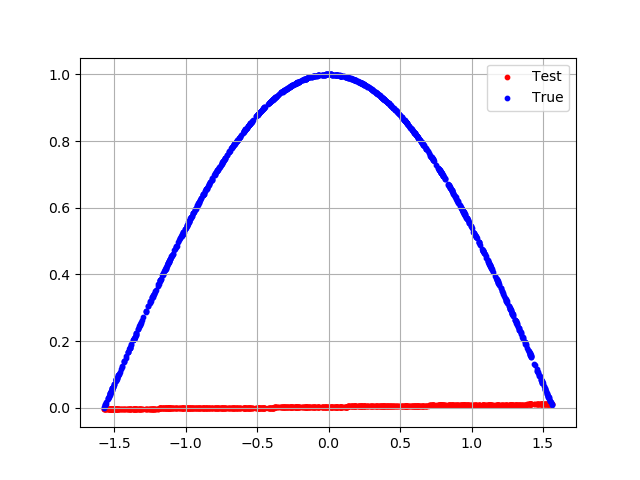
\includegraphics[width=0.3\textwidth]{../width=10loss=mean_squared_errorini=0.01rep=1/predict_plot_0.png}}
				\subfigure[epoch=500]{
					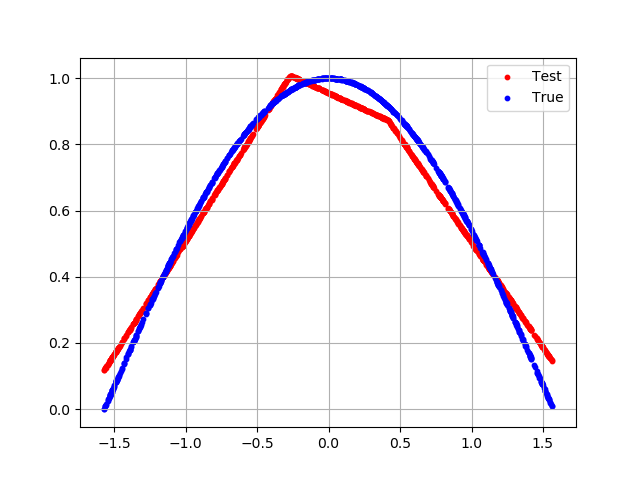
\includegraphics[width=0.3\textwidth]{../width=10loss=mean_squared_errorini=0.01rep=1/predict_plot_500.png}}
				\subfigure[epoch=1000]{
					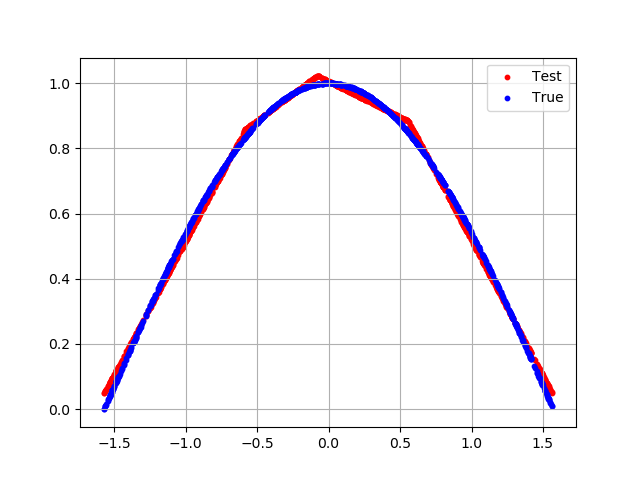
\includegraphics[width=0.3\textwidth]{../width=10loss=mean_squared_errorini=0.01rep=1/predict_plot_1000.png}}
				\subfigure[epoch=1500]{
					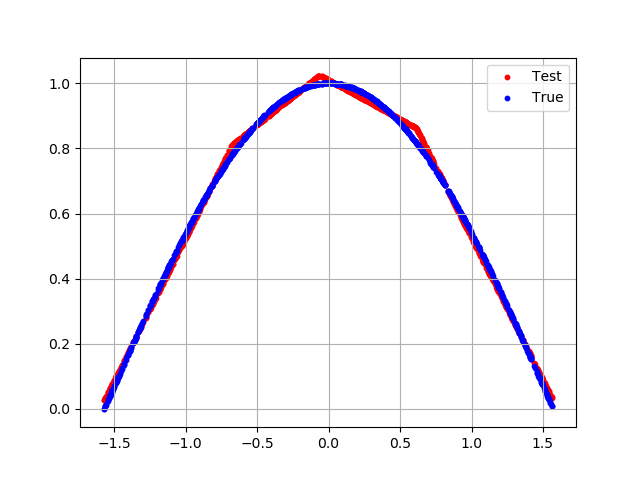
\includegraphics[width=0.3\textwidth]{../width=10loss=mean_squared_errorini=0.01rep=1/predict_plot_1500.png}}
				\subfigure[epoch=2000]{
					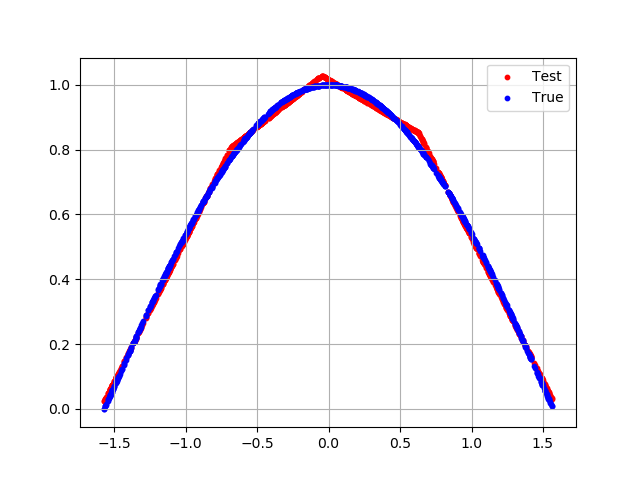
\includegraphics[width=0.3\textwidth]{../width=10loss=mean_squared_errorini=0.01rep=1/predict_plot_2000.png}}
				\subfigure[epoch=2500]{
					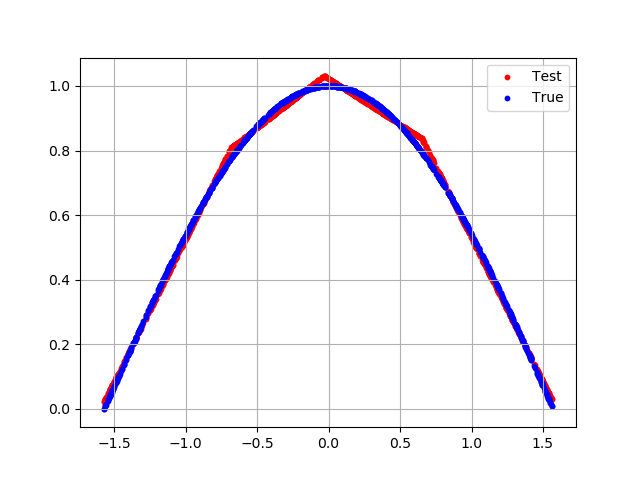
\includegraphics[width=0.3\textwidth]{../width=10loss=mean_squared_errorini=0.01rep=1/predict_plot_2500.png}}
				\subfigure[Loss vs. epoch]{
					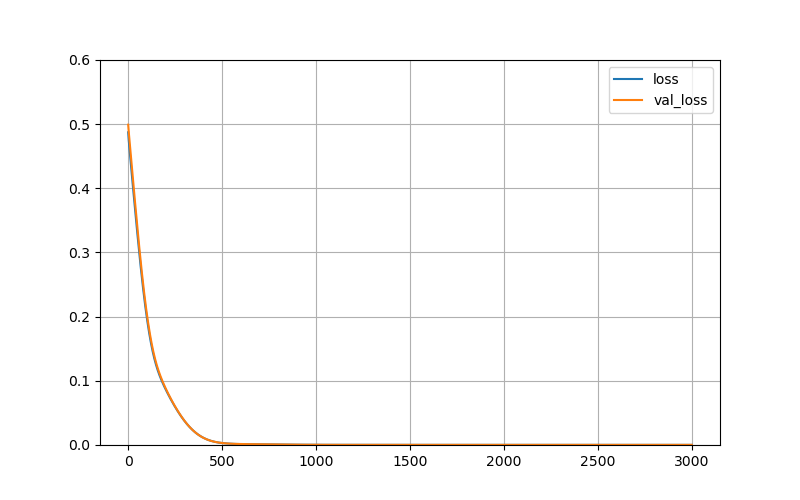
\includegraphics[width=0.6\linewidth]{../width=10loss=mean_squared_errorini=0.01rep=1/learning_curve.png}}
				\caption{Curve Fitting Process(experiment 1)}
			\end{figure}
			\newpage

			\begin{figure}[h]
				\centering  
				\subfigure[epoch=0]{
					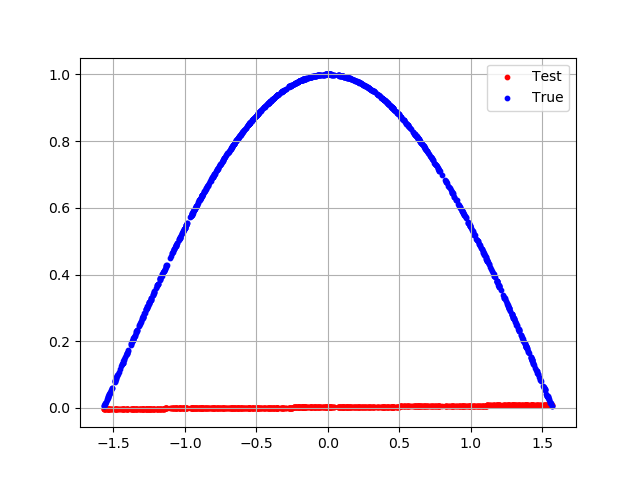
\includegraphics[width=0.3\textwidth]{../width=10loss=mean_squared_errorini=0.01rep=2/predict_plot_0.png}}
				\subfigure[epoch=500]{
					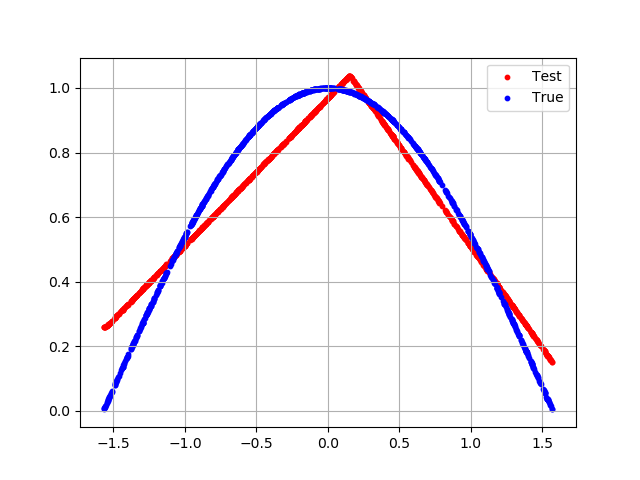
\includegraphics[width=0.3\textwidth]{../width=10loss=mean_squared_errorini=0.01rep=2/predict_plot_500.png}}
				\subfigure[epoch=1000]{
					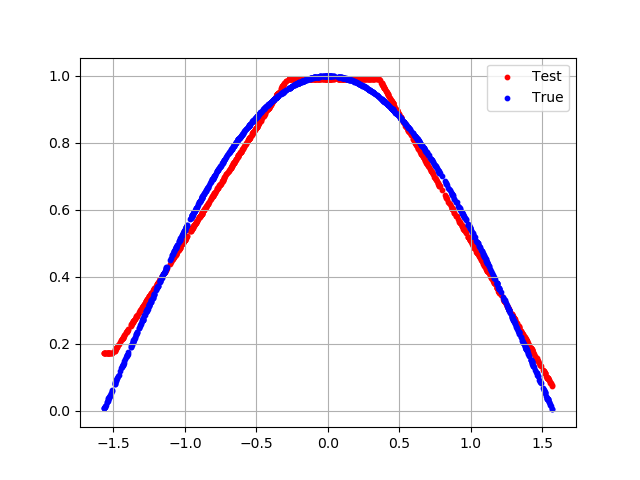
\includegraphics[width=0.3\textwidth]{../width=10loss=mean_squared_errorini=0.01rep=2/predict_plot_1000.png}}
				\subfigure[epoch=1500]{
					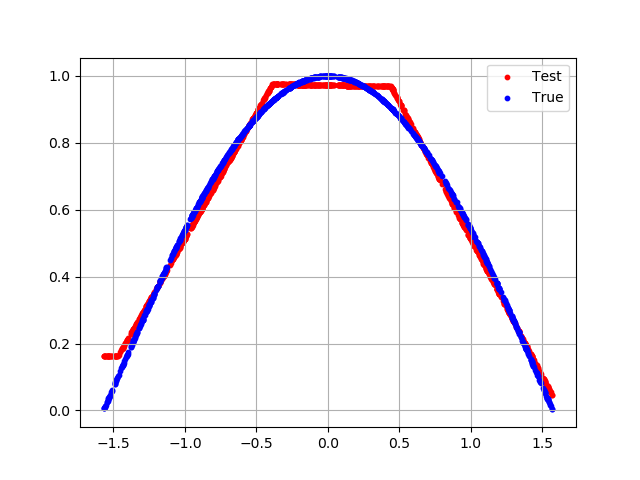
\includegraphics[width=0.3\textwidth]{../width=10loss=mean_squared_errorini=0.01rep=2/predict_plot_1500.png}}
				\subfigure[epoch=2000]{
					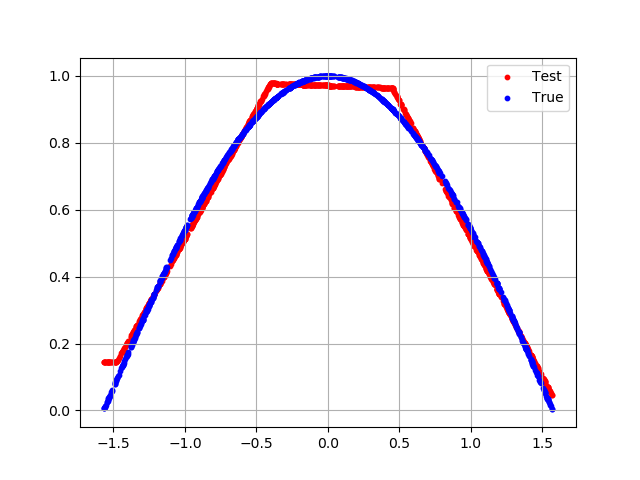
\includegraphics[width=0.3\textwidth]{../width=10loss=mean_squared_errorini=0.01rep=2/predict_plot_2000.png}}
				\subfigure[epoch=2500]{
					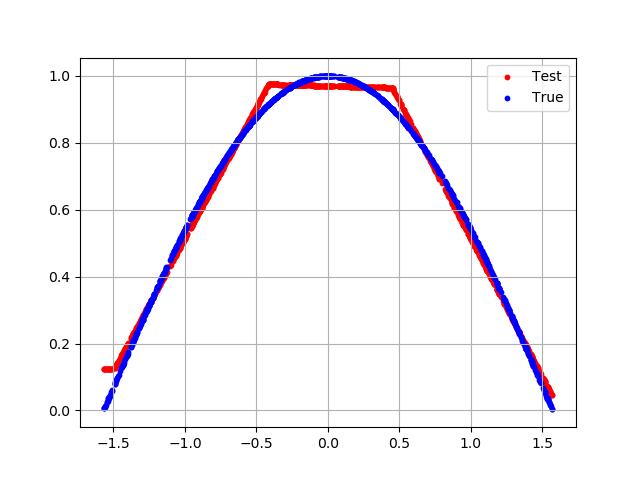
\includegraphics[width=0.3\textwidth]{../width=10loss=mean_squared_errorini=0.01rep=2/predict_plot_2500.png}}
				\subfigure[Loss vs. epoch]{
					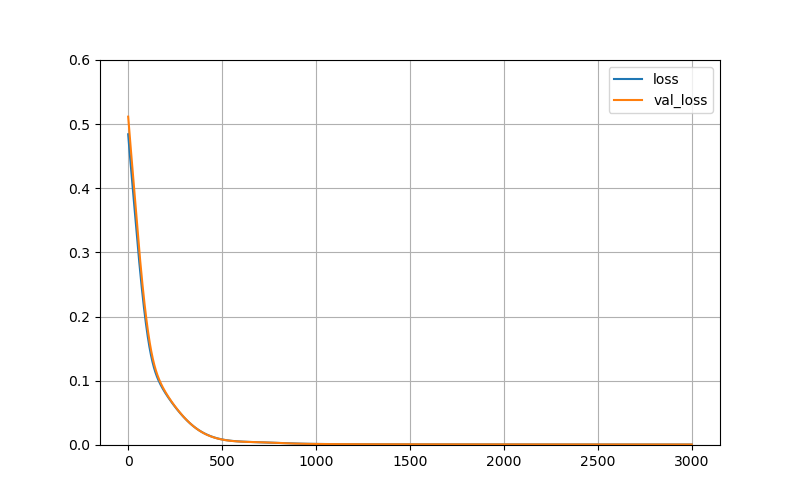
\includegraphics[width=0.6\linewidth]{../width=10loss=mean_squared_errorini=0.01rep=2/learning_curve.png}}
				\caption{Curve Fitting Process(experiment 2)}
			\end{figure}
			\newpage

			\begin{figure}[h]
				\centering  
				\subfigure[epoch=0]{
					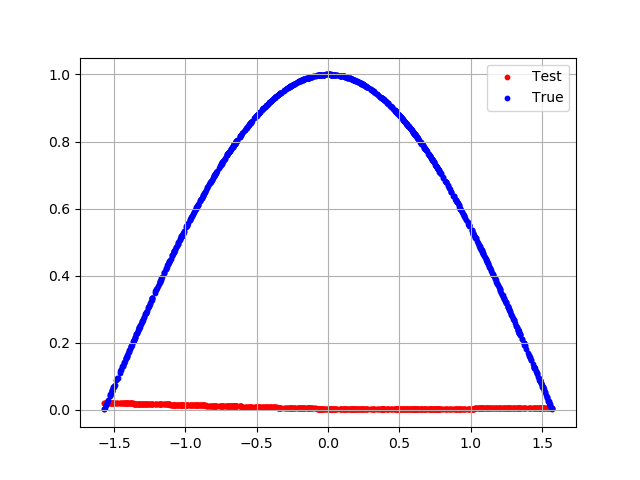
\includegraphics[width=0.3\textwidth]{../width=10loss=mean_squared_errorini=0.01rep=3/predict_plot_0.png}}
				\subfigure[epoch=500]{
					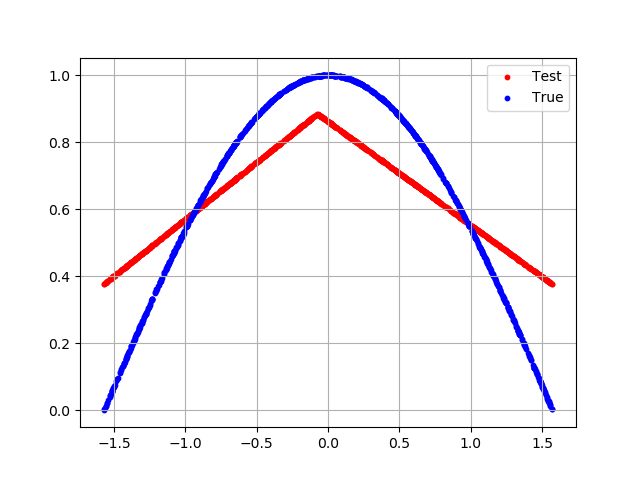
\includegraphics[width=0.3\textwidth]{../width=10loss=mean_squared_errorini=0.01rep=3/predict_plot_500.png}}
				\subfigure[epoch=1000]{
					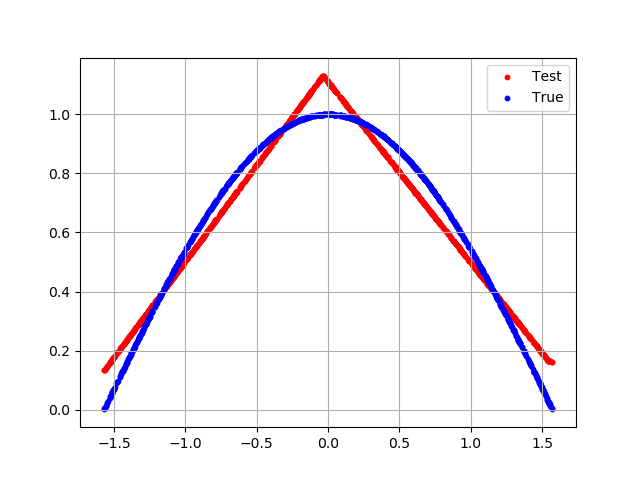
\includegraphics[width=0.3\textwidth]{../width=10loss=mean_squared_errorini=0.01rep=3/predict_plot_1000.png}}
				\subfigure[epoch=1500]{
					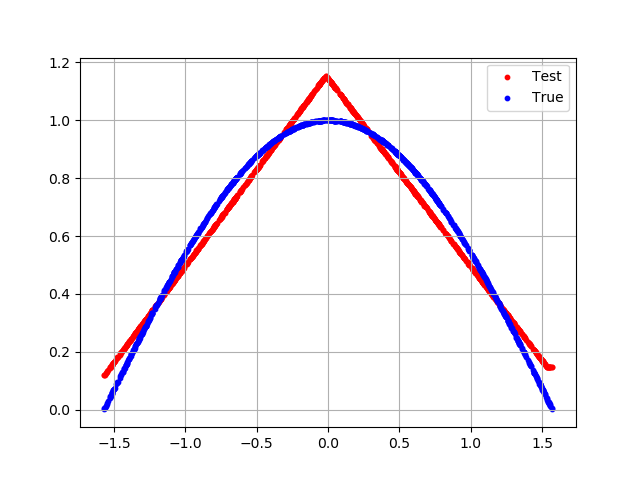
\includegraphics[width=0.3\textwidth]{../width=10loss=mean_squared_errorini=0.01rep=3/predict_plot_1500.png}}
				\subfigure[epoch=2000]{
					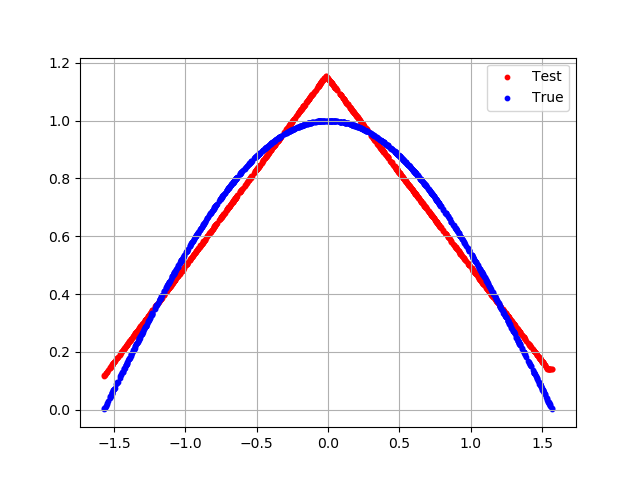
\includegraphics[width=0.3\textwidth]{../width=10loss=mean_squared_errorini=0.01rep=3/predict_plot_2000.png}}
				\subfigure[epoch=2500]{
					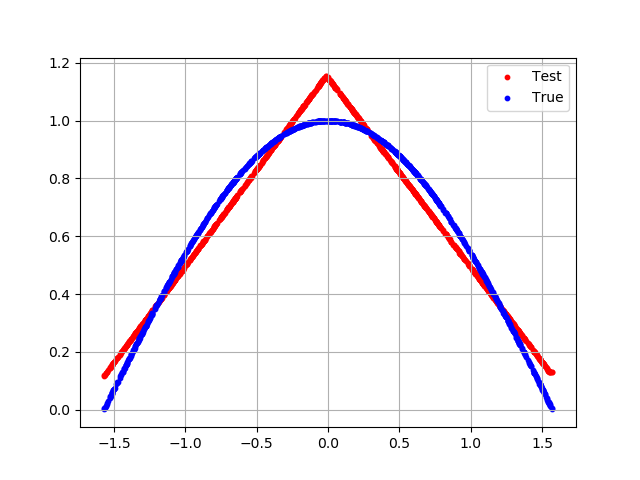
\includegraphics[width=0.3\textwidth]{../width=10loss=mean_squared_errorini=0.01rep=3/predict_plot_2500.png}}
				\subfigure[Loss vs. epoch]{
					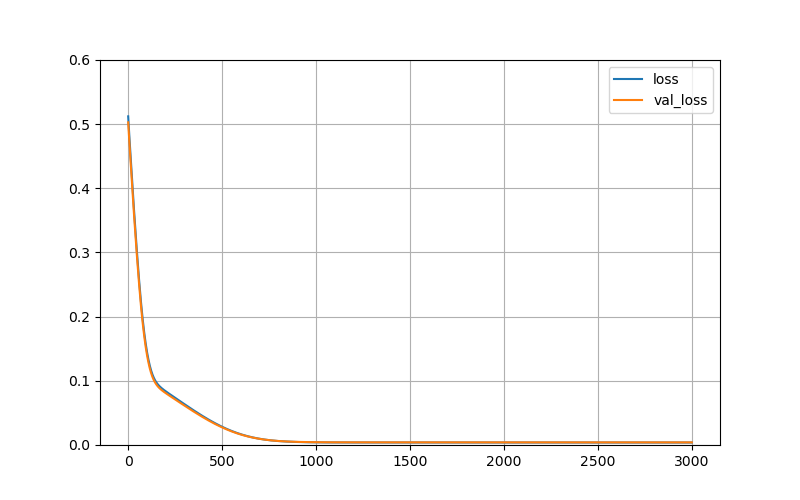
\includegraphics[width=0.6\linewidth]{../width=10loss=mean_squared_errorini=0.01rep=3/learning_curve.png}}
				\caption{Curve Fitting Process(experiment 3)}
			\end{figure}
			\newpage

			\begin{figure}[h]
				\centering  
				\subfigure[epoch=0]{
					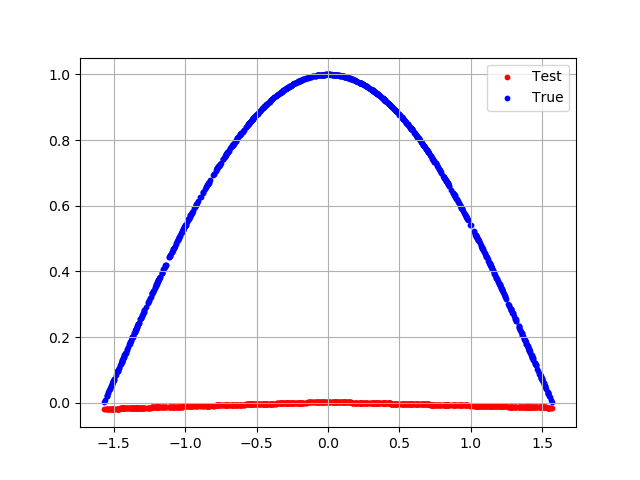
\includegraphics[width=0.3\textwidth]{../width=10loss=mean_squared_errorini=0.01rep=4/predict_plot_0.png}}
				\subfigure[epoch=500]{
					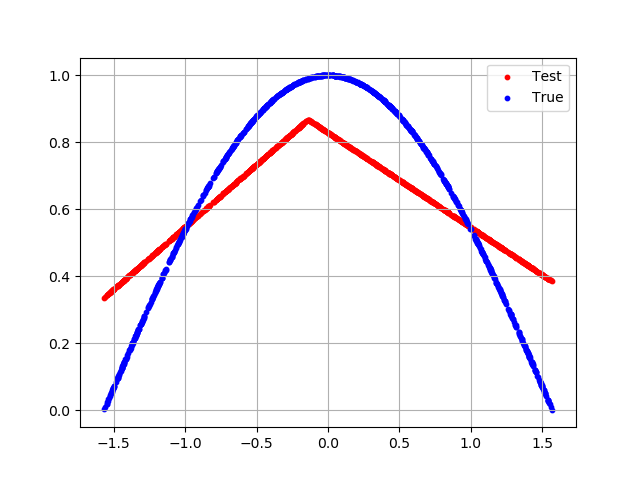
\includegraphics[width=0.3\textwidth]{../width=10loss=mean_squared_errorini=0.01rep=4/predict_plot_500.png}}
				\subfigure[epoch=1000]{
					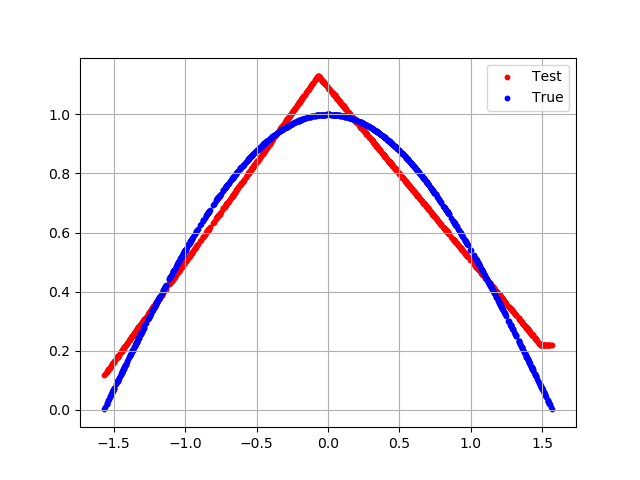
\includegraphics[width=0.3\textwidth]{../width=10loss=mean_squared_errorini=0.01rep=4/predict_plot_1000.png}}
				\subfigure[epoch=1500]{
					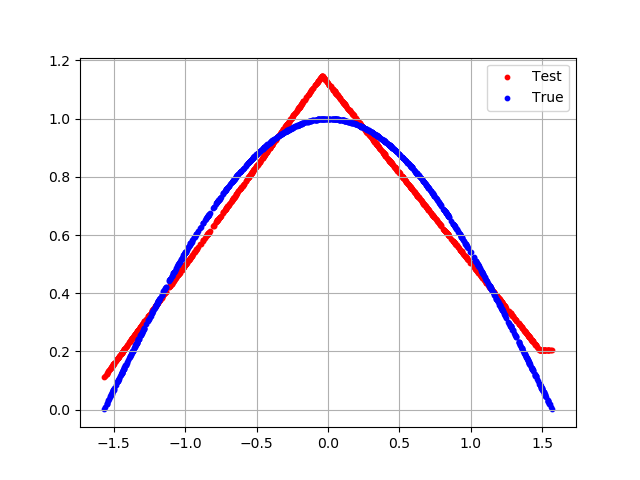
\includegraphics[width=0.3\textwidth]{../width=10loss=mean_squared_errorini=0.01rep=4/predict_plot_1500.png}}
				\subfigure[epoch=2000]{
					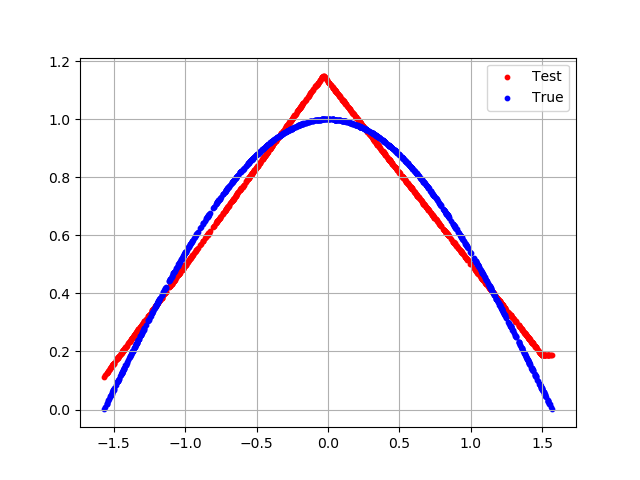
\includegraphics[width=0.3\textwidth]{../width=10loss=mean_squared_errorini=0.01rep=4/predict_plot_2000.png}}
				\subfigure[epoch=2500]{
					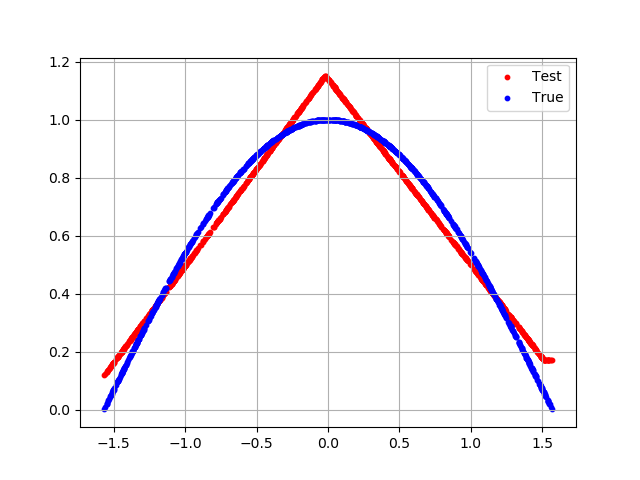
\includegraphics[width=0.3\textwidth]{../width=10loss=mean_squared_errorini=0.01rep=4/predict_plot_2500.png}}
				\subfigure[Loss vs. epoch]{
					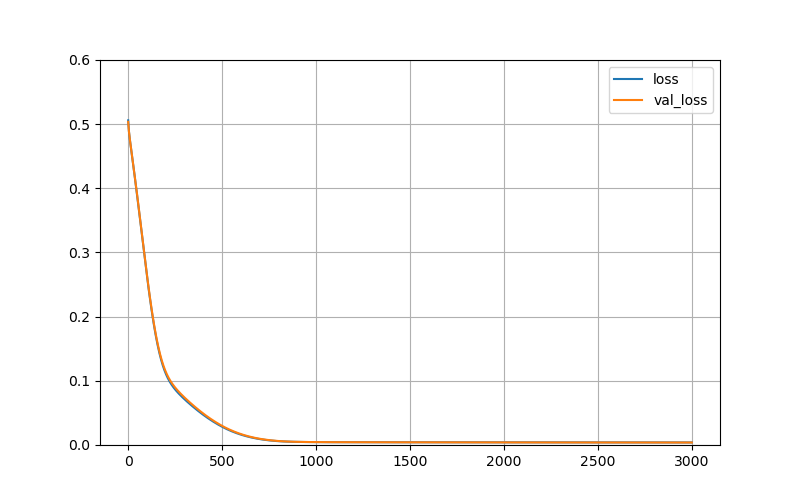
\includegraphics[width=0.6\linewidth]{../width=10loss=mean_squared_errorini=0.01rep=4/learning_curve.png}}
				\caption{Curve Fitting Process(experiment 4)}
			\end{figure}
			\newpage

			\subsubsection{Standard Error = 0.1}
				\begin{figure}[h]
					\centering  
					\subfigure[epoch=0]{
						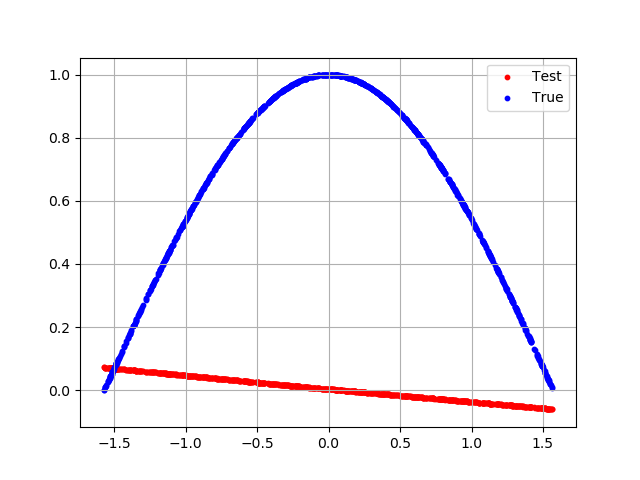
\includegraphics[width=0.3\textwidth]{../width=10loss=mean_squared_errorini=0.1rep=1/predict_plot_0.png}}
					\subfigure[epoch=500]{
						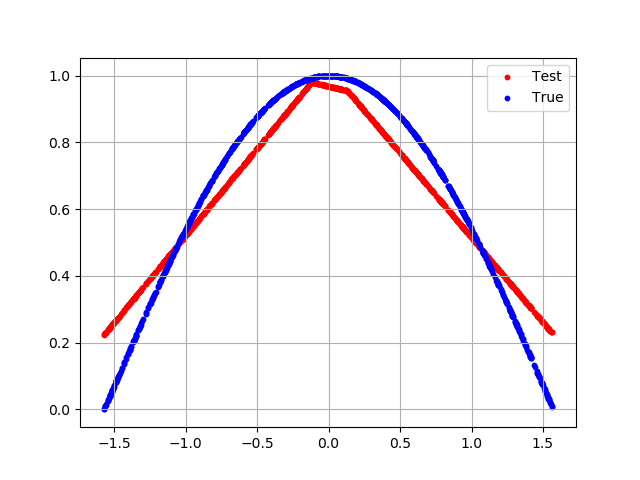
\includegraphics[width=0.3\textwidth]{../width=10loss=mean_squared_errorini=0.1rep=1/predict_plot_500.png}}
					\subfigure[epoch=1000]{
						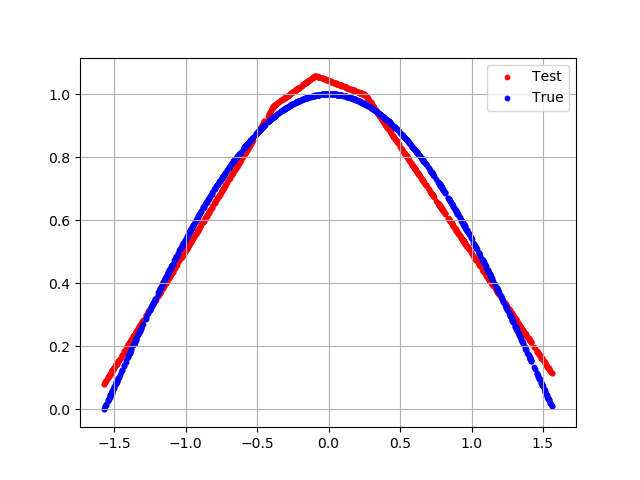
\includegraphics[width=0.3\textwidth]{../width=10loss=mean_squared_errorini=0.1rep=1/predict_plot_1000.png}}
					\subfigure[epoch=1500]{
						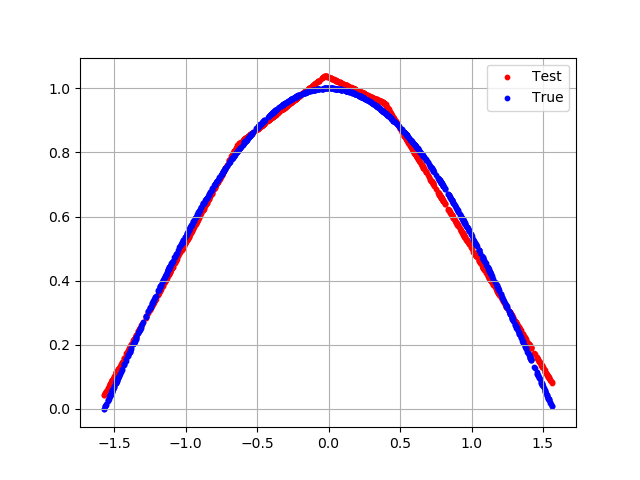
\includegraphics[width=0.3\textwidth]{../width=10loss=mean_squared_errorini=0.1rep=1/predict_plot_1500.png}}
					\subfigure[epoch=2000]{
						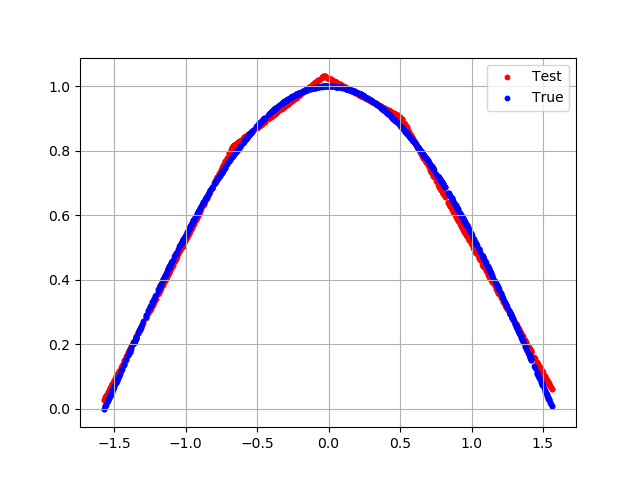
\includegraphics[width=0.3\textwidth]{../width=10loss=mean_squared_errorini=0.1rep=1/predict_plot_2000.png}}
					\subfigure[epoch=2500]{
						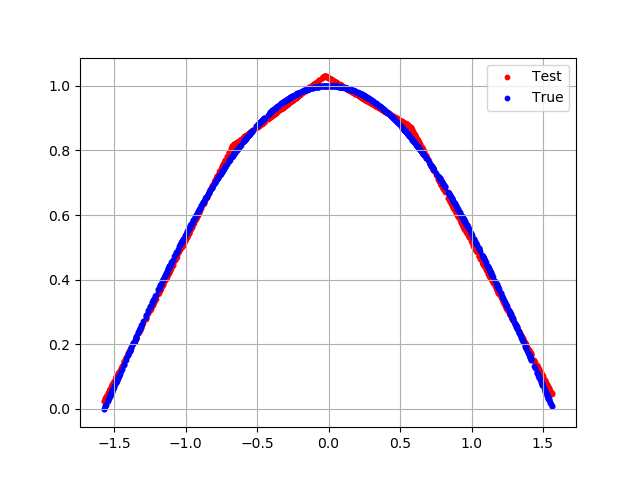
\includegraphics[width=0.3\textwidth]{../width=10loss=mean_squared_errorini=0.1rep=1/predict_plot_2500.png}}
					\subfigure[Loss vs. epoch]{
						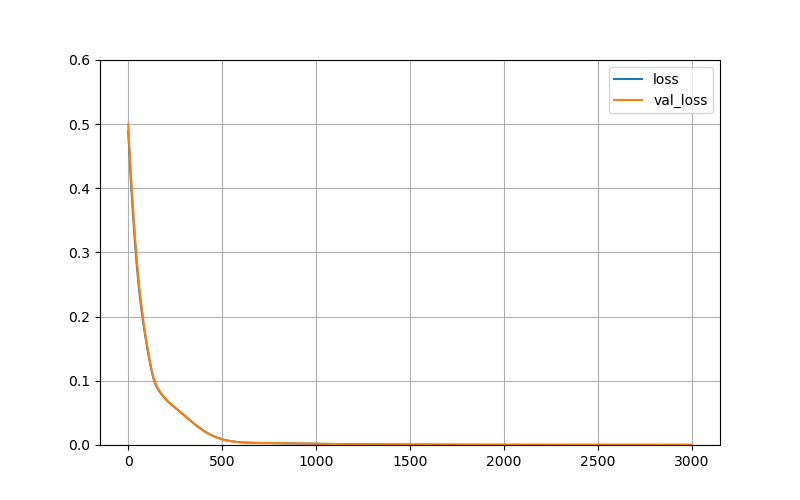
\includegraphics[width=0.6\linewidth]{../width=10loss=mean_squared_errorini=0.1rep=1/learning_curve.png}}
					\caption{Curve Fitting Process(experiment 1)}
				\end{figure}
				\newpage

				\begin{figure}[h]
					\centering  
					\subfigure[epoch=0]{
						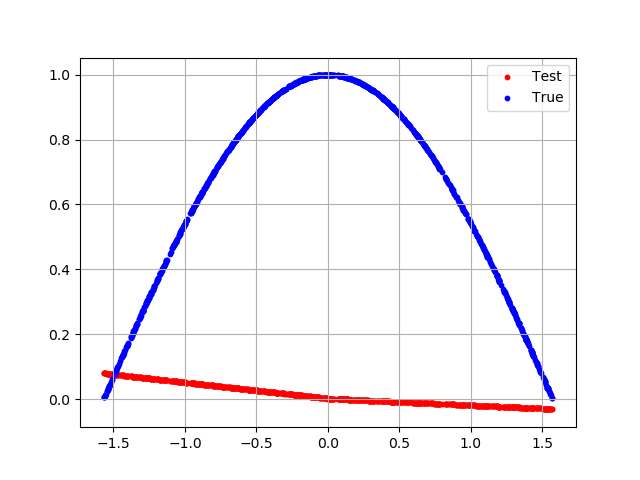
\includegraphics[width=0.3\textwidth]{../width=10loss=mean_squared_errorini=0.1rep=2/predict_plot_0.png}}
					\subfigure[epoch=500]{
						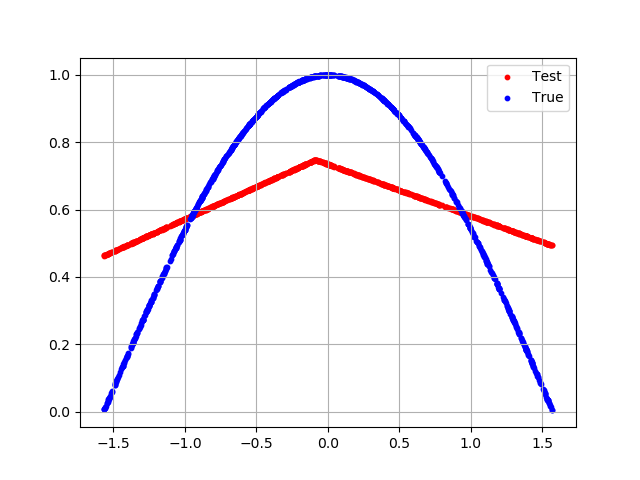
\includegraphics[width=0.3\textwidth]{../width=10loss=mean_squared_errorini=0.1rep=2/predict_plot_500.png}}
					\subfigure[epoch=1000]{
						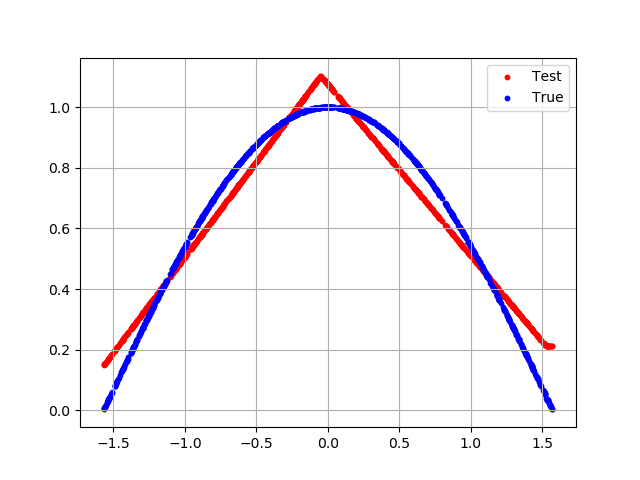
\includegraphics[width=0.3\textwidth]{../width=10loss=mean_squared_errorini=0.1rep=2/predict_plot_1000.png}}
					\subfigure[epoch=1500]{
						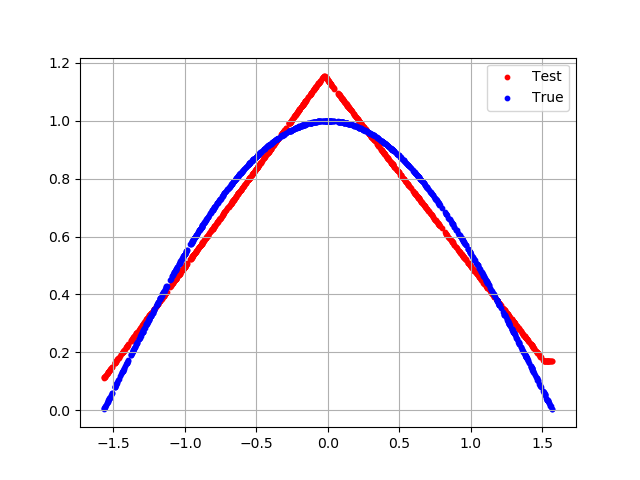
\includegraphics[width=0.3\textwidth]{../width=10loss=mean_squared_errorini=0.1rep=2/predict_plot_1500.png}}
					\subfigure[epoch=2000]{
						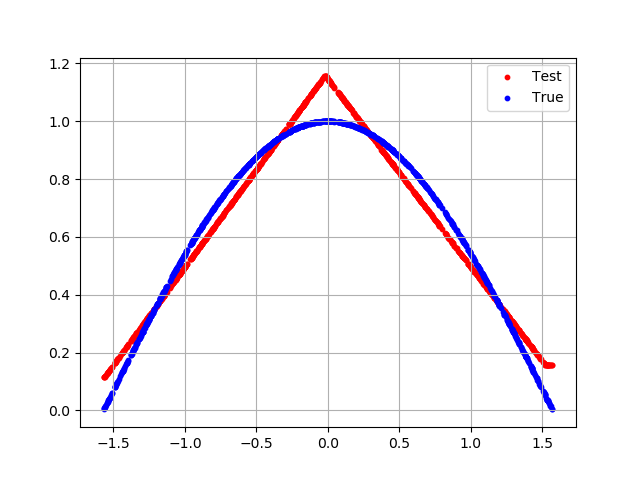
\includegraphics[width=0.3\textwidth]{../width=10loss=mean_squared_errorini=0.1rep=2/predict_plot_2000.png}}
					\subfigure[epoch=2500]{
						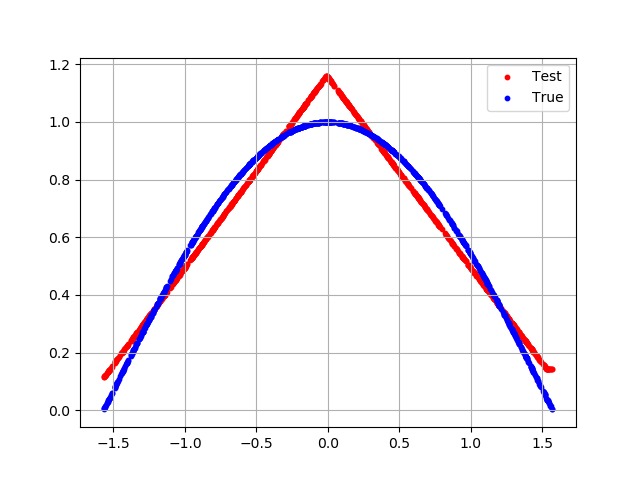
\includegraphics[width=0.3\textwidth]{../width=10loss=mean_squared_errorini=0.1rep=2/predict_plot_2500.png}}
					\subfigure[Loss vs. epoch]{
						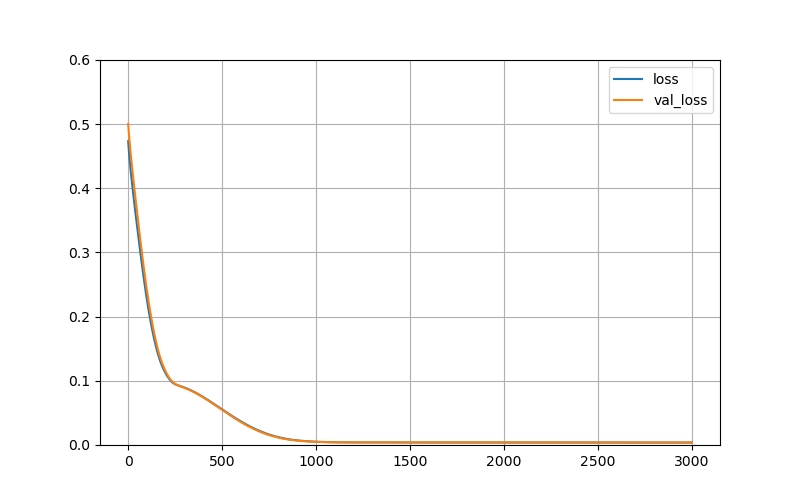
\includegraphics[width=0.6\linewidth]{../width=10loss=mean_squared_errorini=0.1rep=2/learning_curve.png}}
					\caption{Curve Fitting Process(experiment 2)}
				\end{figure}
				\newpage

				\begin{figure}[h]
					\centering  
					\subfigure[epoch=0]{
						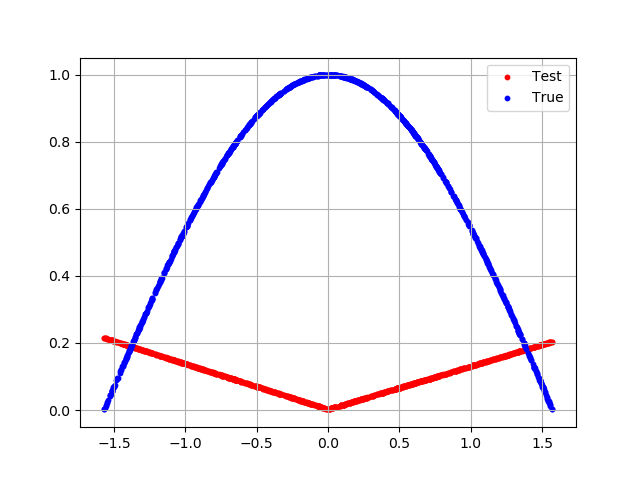
\includegraphics[width=0.3\textwidth]{../width=10loss=mean_squared_errorini=0.1rep=3/predict_plot_0.png}}
					\subfigure[epoch=500]{
						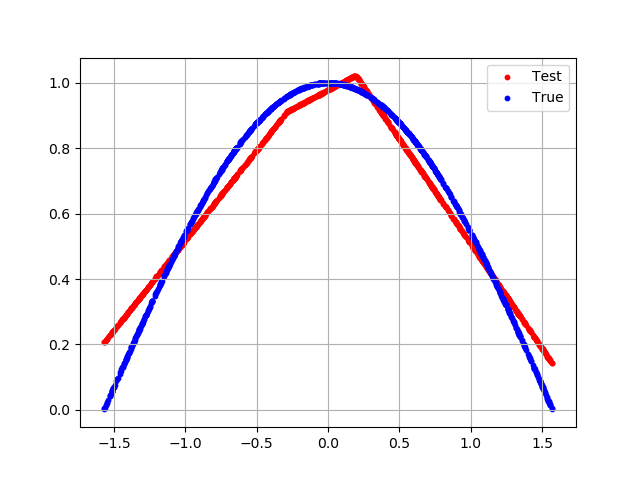
\includegraphics[width=0.3\textwidth]{../width=10loss=mean_squared_errorini=0.1rep=3/predict_plot_500.png}}
					\subfigure[epoch=1000]{
						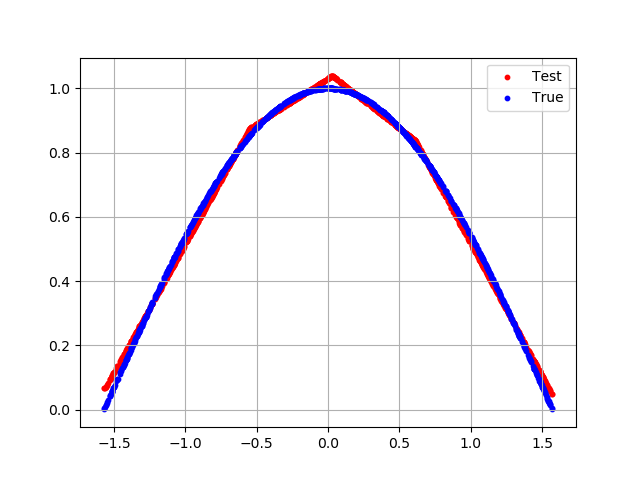
\includegraphics[width=0.3\textwidth]{../width=10loss=mean_squared_errorini=0.1rep=3/predict_plot_1000.png}}
					\subfigure[epoch=1500]{
						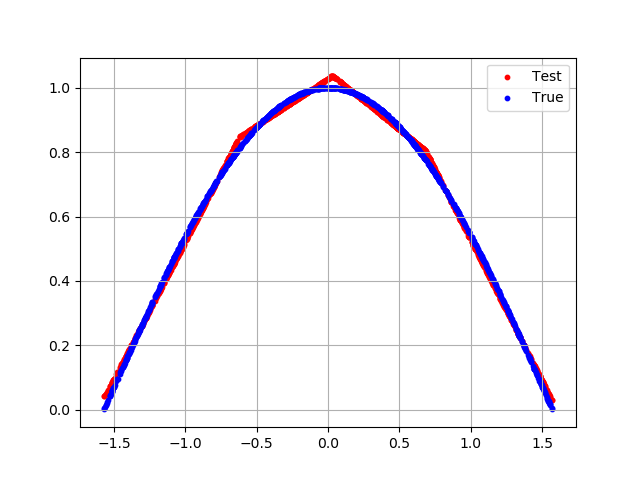
\includegraphics[width=0.3\textwidth]{../width=10loss=mean_squared_errorini=0.1rep=3/predict_plot_1500.png}}
					\subfigure[epoch=2000]{
						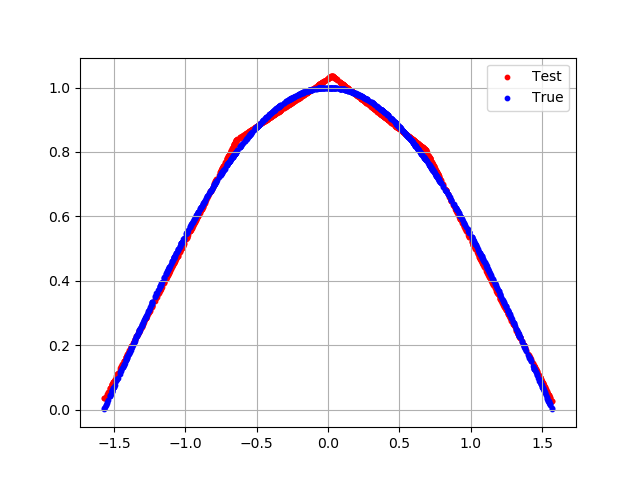
\includegraphics[width=0.3\textwidth]{../width=10loss=mean_squared_errorini=0.1rep=3/predict_plot_2000.png}}
					\subfigure[epoch=2500]{
						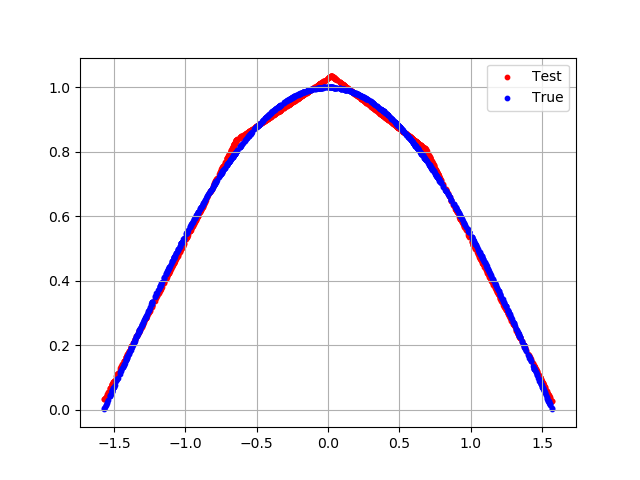
\includegraphics[width=0.3\textwidth]{../width=10loss=mean_squared_errorini=0.1rep=3/predict_plot_2500.png}}
					\subfigure[Loss vs. epoch]{
						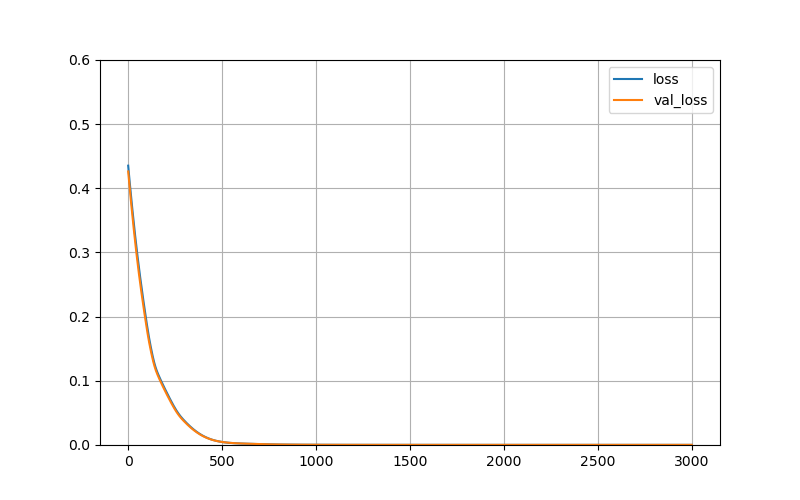
\includegraphics[width=0.6\linewidth]{../width=10loss=mean_squared_errorini=0.1rep=3/learning_curve.png}}
					\caption{Curve Fitting Process(experiment 3)}
				\end{figure}
				\newpage

				\begin{figure}[h]
					\centering  
					\subfigure[epoch=0]{
						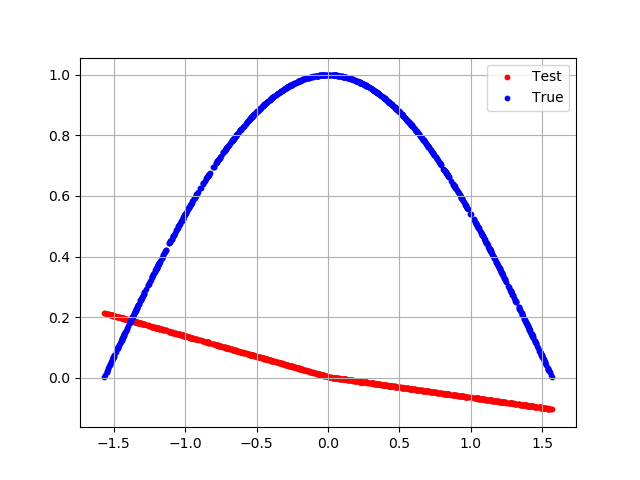
\includegraphics[width=0.3\textwidth]{../width=10loss=mean_squared_errorini=0.1rep=4/predict_plot_0.png}}
					\subfigure[epoch=500]{
						\includegraphics[width=0.3\textwidth]{../width=10loss=mean_squared_errorini=0.1rep=4/predict_plot_500.png}}
					\subfigure[epoch=1000]{
						\includegraphics[width=0.3\textwidth]{../width=10loss=mean_squared_errorini=0.1rep=4/predict_plot_1000.png}}
					\subfigure[epoch=1500]{
						\includegraphics[width=0.3\textwidth]{../width=10loss=mean_squared_errorini=0.1rep=4/predict_plot_1500.png}}
					\subfigure[epoch=2000]{
						\includegraphics[width=0.3\textwidth]{../width=10loss=mean_squared_errorini=0.1rep=4/predict_plot_2000.png}}
					\subfigure[epoch=2500]{
						\includegraphics[width=0.3\textwidth]{../width=10loss=mean_squared_errorini=0.1rep=4/predict_plot_2500.png}}
					\subfigure[Loss vs. epoch]{
						\includegraphics[width=0.6\linewidth]{../width=10loss=mean_squared_errorini=0.1rep=4/learning_curve.png}}
					\caption{Curve Fitting Process(experiment 4)}
				\end{figure}
				\newpage


			\subsubsection{Standard Error = 1}
				\begin{figure}[h]
					\centering  
					\subfigure[epoch=0]{
						\includegraphics[width=0.3\textwidth]{../width=10loss=mean_squared_errorini=1rep=1/predict_plot_0.png}}
					\subfigure[epoch=500]{
						\includegraphics[width=0.3\textwidth]{../width=10loss=mean_squared_errorini=1rep=1/predict_plot_500.png}}
					\subfigure[epoch=1000]{
						\includegraphics[width=0.3\textwidth]{../width=10loss=mean_squared_errorini=1rep=1/predict_plot_1000.png}}
					\subfigure[epoch=1500]{
						\includegraphics[width=0.3\textwidth]{../width=10loss=mean_squared_errorini=1rep=1/predict_plot_1500.png}}
					\subfigure[epoch=2000]{
						\includegraphics[width=0.3\textwidth]{../width=10loss=mean_squared_errorini=1rep=1/predict_plot_2000.png}}
					\subfigure[epoch=2500]{
						\includegraphics[width=0.3\textwidth]{../width=10loss=mean_squared_errorini=1rep=1/predict_plot_2500.png}}
					\subfigure[Loss vs. epoch]{
						\includegraphics[width=0.6\linewidth]{../width=10loss=mean_squared_errorini=1rep=1/learning_curve.png}}
					\caption{Curve Fitting Process(experiment 1)}
				\end{figure}
				\newpage

				\begin{figure}[h]
					\centering  
					\subfigure[epoch=0]{
						\includegraphics[width=0.3\textwidth]{../width=10loss=mean_squared_errorini=1rep=2/predict_plot_0.png}}
					\subfigure[epoch=500]{
						\includegraphics[width=0.3\textwidth]{../width=10loss=mean_squared_errorini=1rep=2/predict_plot_500.png}}
					\subfigure[epoch=1000]{
						\includegraphics[width=0.3\textwidth]{../width=10loss=mean_squared_errorini=1rep=2/predict_plot_1000.png}}
					\subfigure[epoch=1500]{
						\includegraphics[width=0.3\textwidth]{../width=10loss=mean_squared_errorini=1rep=2/predict_plot_1500.png}}
					\subfigure[epoch=2000]{
						\includegraphics[width=0.3\textwidth]{../width=10loss=mean_squared_errorini=1rep=2/predict_plot_2000.png}}
					\subfigure[epoch=2500]{
						\includegraphics[width=0.3\textwidth]{../width=10loss=mean_squared_errorini=1rep=2/predict_plot_2500.png}}
					\subfigure[Loss vs. epoch]{
						\includegraphics[width=0.6\linewidth]{../width=10loss=mean_squared_errorini=1rep=2/learning_curve.png}}
					\caption{Curve Fitting Process(experiment 2)}
				\end{figure}
				\newpage

				\begin{figure}[h]
					\centering  
					\subfigure[epoch=0]{
						\includegraphics[width=0.3\textwidth]{../width=10loss=mean_squared_errorini=1rep=3/predict_plot_0.png}}
					\subfigure[epoch=500]{
						\includegraphics[width=0.3\textwidth]{../width=10loss=mean_squared_errorini=1rep=3/predict_plot_500.png}}
					\subfigure[epoch=1000]{
						\includegraphics[width=0.3\textwidth]{../width=10loss=mean_squared_errorini=1rep=3/predict_plot_1000.png}}
					\subfigure[epoch=1500]{
						\includegraphics[width=0.3\textwidth]{../width=10loss=mean_squared_errorini=1rep=3/predict_plot_1500.png}}
					\subfigure[epoch=2000]{
						\includegraphics[width=0.3\textwidth]{../width=10loss=mean_squared_errorini=1rep=3/predict_plot_2000.png}}
					\subfigure[epoch=2500]{
						\includegraphics[width=0.3\textwidth]{../width=10loss=mean_squared_errorini=1rep=3/predict_plot_2500.png}}
					\subfigure[Loss vs. epoch]{
						\includegraphics[width=0.6\linewidth]{../width=10loss=mean_squared_errorini=1rep=3/learning_curve.png}}
					\caption{Curve Fitting Process(experiment 3)}
				\end{figure}
				\newpage

				\begin{figure}[h]
					\centering  
					\subfigure[epoch=0]{
						\includegraphics[width=0.3\textwidth]{../width=10loss=mean_squared_errorini=1rep=4/predict_plot_0.png}}
					\subfigure[epoch=500]{
						\includegraphics[width=0.3\textwidth]{../width=10loss=mean_squared_errorini=1rep=4/predict_plot_500.png}}
					\subfigure[epoch=1000]{
						\includegraphics[width=0.3\textwidth]{../width=10loss=mean_squared_errorini=1rep=4/predict_plot_1000.png}}
					\subfigure[epoch=1500]{
						\includegraphics[width=0.3\textwidth]{../width=10loss=mean_squared_errorini=1rep=4/predict_plot_1500.png}}
					\subfigure[epoch=2000]{
						\includegraphics[width=0.3\textwidth]{../width=10loss=mean_squared_errorini=1rep=4/predict_plot_2000.png}}
					\subfigure[epoch=2500]{
						\includegraphics[width=0.3\textwidth]{../width=10loss=mean_squared_errorini=1rep=4/predict_plot_2500.png}}
					\subfigure[Loss vs. epoch]{
						\includegraphics[width=0.6\linewidth]{../width=10loss=mean_squared_errorini=1rep=4/learning_curve.png}}
					\caption{Curve Fitting Process(experiment 4)}
				\end{figure}
				\newpage



			\subsection{Mean Absolute Error}
				\subsubsection{Standard Error = 0.01}
			
				\begin{figure}[h]
					\centering  
					\subfigure[epoch=0]{
						\includegraphics[width=0.3\textwidth]{../width=10loss=mean_absolute_errorini=0.01rep=1/predict_plot_0.png}}
					\subfigure[epoch=500]{
						\includegraphics[width=0.3\textwidth]{../width=10loss=mean_absolute_errorini=0.01rep=1/predict_plot_500.png}}
					\subfigure[epoch=1000]{
						\includegraphics[width=0.3\textwidth]{../width=10loss=mean_absolute_errorini=0.01rep=1/predict_plot_1000.png}}
					\subfigure[epoch=1500]{
						\includegraphics[width=0.3\textwidth]{../width=10loss=mean_absolute_errorini=0.01rep=1/predict_plot_1500.png}}
					\subfigure[epoch=2000]{
						\includegraphics[width=0.3\textwidth]{../width=10loss=mean_absolute_errorini=0.01rep=1/predict_plot_2000.png}}
					\subfigure[epoch=2500]{
						\includegraphics[width=0.3\textwidth]{../width=10loss=mean_absolute_errorini=0.01rep=1/predict_plot_2500.png}}
					\subfigure[Loss vs. epoch]{
						\includegraphics[width=0.6\linewidth]{../width=10loss=mean_absolute_errorini=0.01rep=1/learning_curve.png}}
					\caption{Curve Fitting Process(experiment 1)}
				\end{figure}
				\newpage
	
				\begin{figure}[h]
					\centering  
					\subfigure[epoch=0]{
						\includegraphics[width=0.3\textwidth]{../width=10loss=mean_absolute_errorini=0.01rep=2/predict_plot_0.png}}
					\subfigure[epoch=500]{
						\includegraphics[width=0.3\textwidth]{../width=10loss=mean_absolute_errorini=0.01rep=2/predict_plot_500.png}}
					\subfigure[epoch=1000]{
						\includegraphics[width=0.3\textwidth]{../width=10loss=mean_absolute_errorini=0.01rep=2/predict_plot_1000.png}}
					\subfigure[epoch=1500]{
						\includegraphics[width=0.3\textwidth]{../width=10loss=mean_absolute_errorini=0.01rep=2/predict_plot_1500.png}}
					\subfigure[epoch=2000]{
						\includegraphics[width=0.3\textwidth]{../width=10loss=mean_absolute_errorini=0.01rep=2/predict_plot_2000.png}}
					\subfigure[epoch=2500]{
						\includegraphics[width=0.3\textwidth]{../width=10loss=mean_absolute_errorini=0.01rep=2/predict_plot_2500.png}}
					\subfigure[Loss vs. epoch]{
						\includegraphics[width=0.6\linewidth]{../width=10loss=mean_absolute_errorini=0.01rep=2/learning_curve.png}}
					\caption{Curve Fitting Process(experiment 2)}
				\end{figure}
				\newpage
	
				\begin{figure}[h]
					\centering  
					\subfigure[epoch=0]{
						\includegraphics[width=0.3\textwidth]{../width=10loss=mean_absolute_errorini=0.01rep=3/predict_plot_0.png}}
					\subfigure[epoch=500]{
						\includegraphics[width=0.3\textwidth]{../width=10loss=mean_absolute_errorini=0.01rep=3/predict_plot_500.png}}
					\subfigure[epoch=1000]{
						\includegraphics[width=0.3\textwidth]{../width=10loss=mean_absolute_errorini=0.01rep=3/predict_plot_1000.png}}
					\subfigure[epoch=1500]{
						\includegraphics[width=0.3\textwidth]{../width=10loss=mean_absolute_errorini=0.01rep=3/predict_plot_1500.png}}
					\subfigure[epoch=2000]{
						\includegraphics[width=0.3\textwidth]{../width=10loss=mean_absolute_errorini=0.01rep=3/predict_plot_2000.png}}
					\subfigure[epoch=2500]{
						\includegraphics[width=0.3\textwidth]{../width=10loss=mean_absolute_errorini=0.01rep=3/predict_plot_2500.png}}
					\subfigure[Loss vs. epoch]{
						\includegraphics[width=0.6\linewidth]{../width=10loss=mean_absolute_errorini=0.01rep=3/learning_curve.png}}
					\caption{Curve Fitting Process(experiment 3)}
				\end{figure}
				\newpage
	
				\begin{figure}[h]
					\centering  
					\subfigure[epoch=0]{
						\includegraphics[width=0.3\textwidth]{../width=10loss=mean_absolute_errorini=0.01rep=4/predict_plot_0.png}}
					\subfigure[epoch=500]{
						\includegraphics[width=0.3\textwidth]{../width=10loss=mean_absolute_errorini=0.01rep=4/predict_plot_500.png}}
					\subfigure[epoch=1000]{
						\includegraphics[width=0.3\textwidth]{../width=10loss=mean_absolute_errorini=0.01rep=4/predict_plot_1000.png}}
					\subfigure[epoch=1500]{
						\includegraphics[width=0.3\textwidth]{../width=10loss=mean_absolute_errorini=0.01rep=4/predict_plot_1500.png}}
					\subfigure[epoch=2000]{
						\includegraphics[width=0.3\textwidth]{../width=10loss=mean_absolute_errorini=0.01rep=4/predict_plot_2000.png}}
					\subfigure[epoch=2500]{
						\includegraphics[width=0.3\textwidth]{../width=10loss=mean_absolute_errorini=0.01rep=4/predict_plot_2500.png}}
					\subfigure[Loss vs. epoch]{
						\includegraphics[width=0.6\linewidth]{../width=10loss=mean_absolute_errorini=0.01rep=4/learning_curve.png}}
					\caption{Curve Fitting Process(experiment 4)}
				\end{figure}
				\newpage
	
				\subsubsection{Standard Error = 0.1}
					\begin{figure}[h]
						\centering  
						\subfigure[epoch=0]{
							\includegraphics[width=0.3\textwidth]{../width=10loss=mean_absolute_errorini=0.1rep=1/predict_plot_0.png}}
						\subfigure[epoch=500]{
							\includegraphics[width=0.3\textwidth]{../width=10loss=mean_absolute_errorini=0.1rep=1/predict_plot_500.png}}
						\subfigure[epoch=1000]{
							\includegraphics[width=0.3\textwidth]{../width=10loss=mean_absolute_errorini=0.1rep=1/predict_plot_1000.png}}
						\subfigure[epoch=1500]{
							\includegraphics[width=0.3\textwidth]{../width=10loss=mean_absolute_errorini=0.1rep=1/predict_plot_1500.png}}
						\subfigure[epoch=2000]{
							\includegraphics[width=0.3\textwidth]{../width=10loss=mean_absolute_errorini=0.1rep=1/predict_plot_2000.png}}
						\subfigure[epoch=2500]{
							\includegraphics[width=0.3\textwidth]{../width=10loss=mean_absolute_errorini=0.1rep=1/predict_plot_2500.png}}
						\subfigure[Loss vs. epoch]{
							\includegraphics[width=0.6\linewidth]{../width=10loss=mean_absolute_errorini=0.1rep=1/learning_curve.png}}
						\caption{Curve Fitting Process(experiment 1)}
					\end{figure}
					\newpage
	
					\begin{figure}[h]
						\centering  
						\subfigure[epoch=0]{
							\includegraphics[width=0.3\textwidth]{../width=10loss=mean_absolute_errorini=0.1rep=2/predict_plot_0.png}}
						\subfigure[epoch=500]{
							\includegraphics[width=0.3\textwidth]{../width=10loss=mean_absolute_errorini=0.1rep=2/predict_plot_500.png}}
						\subfigure[epoch=1000]{
							\includegraphics[width=0.3\textwidth]{../width=10loss=mean_absolute_errorini=0.1rep=2/predict_plot_1000.png}}
						\subfigure[epoch=1500]{
							\includegraphics[width=0.3\textwidth]{../width=10loss=mean_absolute_errorini=0.1rep=2/predict_plot_1500.png}}
						\subfigure[epoch=2000]{
							\includegraphics[width=0.3\textwidth]{../width=10loss=mean_absolute_errorini=0.1rep=2/predict_plot_2000.png}}
						\subfigure[epoch=2500]{
							\includegraphics[width=0.3\textwidth]{../width=10loss=mean_absolute_errorini=0.1rep=2/predict_plot_2500.png}}
						\subfigure[Loss vs. epoch]{
							\includegraphics[width=0.6\linewidth]{../width=10loss=mean_absolute_errorini=0.1rep=2/learning_curve.png}}
						\caption{Curve Fitting Process(experiment 2)}
					\end{figure}
					\newpage
	
					\begin{figure}[h]
						\centering  
						\subfigure[epoch=0]{
							\includegraphics[width=0.3\textwidth]{../width=10loss=mean_absolute_errorini=0.1rep=3/predict_plot_0.png}}
						\subfigure[epoch=500]{
							\includegraphics[width=0.3\textwidth]{../width=10loss=mean_absolute_errorini=0.1rep=3/predict_plot_500.png}}
						\subfigure[epoch=1000]{
							\includegraphics[width=0.3\textwidth]{../width=10loss=mean_absolute_errorini=0.1rep=3/predict_plot_1000.png}}
						\subfigure[epoch=1500]{
							\includegraphics[width=0.3\textwidth]{../width=10loss=mean_absolute_errorini=0.1rep=3/predict_plot_1500.png}}
						\subfigure[epoch=2000]{
							\includegraphics[width=0.3\textwidth]{../width=10loss=mean_absolute_errorini=0.1rep=3/predict_plot_2000.png}}
						\subfigure[epoch=2500]{
							\includegraphics[width=0.3\textwidth]{../width=10loss=mean_absolute_errorini=0.1rep=3/predict_plot_2500.png}}
						\subfigure[Loss vs. epoch]{
							\includegraphics[width=0.6\linewidth]{../width=10loss=mean_absolute_errorini=0.1rep=3/learning_curve.png}}
						\caption{Curve Fitting Process(experiment 3)}
					\end{figure}
					\newpage
	
					\begin{figure}[h]
						\centering  
						\subfigure[epoch=0]{
							\includegraphics[width=0.3\textwidth]{../width=10loss=mean_absolute_errorini=0.1rep=4/predict_plot_0.png}}
						\subfigure[epoch=500]{
							\includegraphics[width=0.3\textwidth]{../width=10loss=mean_absolute_errorini=0.1rep=4/predict_plot_500.png}}
						\subfigure[epoch=1000]{
							\includegraphics[width=0.3\textwidth]{../width=10loss=mean_absolute_errorini=0.1rep=4/predict_plot_1000.png}}
						\subfigure[epoch=1500]{
							\includegraphics[width=0.3\textwidth]{../width=10loss=mean_absolute_errorini=0.1rep=4/predict_plot_1500.png}}
						\subfigure[epoch=2000]{
							\includegraphics[width=0.3\textwidth]{../width=10loss=mean_absolute_errorini=0.1rep=4/predict_plot_2000.png}}
						\subfigure[epoch=2500]{
							\includegraphics[width=0.3\textwidth]{../width=10loss=mean_absolute_errorini=0.1rep=4/predict_plot_2500.png}}
						\subfigure[Loss vs. epoch]{
							\includegraphics[width=0.6\linewidth]{../width=10loss=mean_absolute_errorini=0.1rep=4/learning_curve.png}}
						\caption{Curve Fitting Process(experiment 4)}
					\end{figure}
					\newpage
	
	
				\subsubsection{Standard Error = 1}
					\begin{figure}[h]
						\centering  
						\subfigure[epoch=0]{
							\includegraphics[width=0.3\textwidth]{../width=10loss=mean_absolute_errorini=1rep=1/predict_plot_0.png}}
						\subfigure[epoch=500]{
							\includegraphics[width=0.3\textwidth]{../width=10loss=mean_absolute_errorini=1rep=1/predict_plot_500.png}}
						\subfigure[epoch=1000]{
							\includegraphics[width=0.3\textwidth]{../width=10loss=mean_absolute_errorini=1rep=1/predict_plot_1000.png}}
						\subfigure[epoch=1500]{
							\includegraphics[width=0.3\textwidth]{../width=10loss=mean_absolute_errorini=1rep=1/predict_plot_1500.png}}
						\subfigure[epoch=2000]{
							\includegraphics[width=0.3\textwidth]{../width=10loss=mean_absolute_errorini=1rep=1/predict_plot_2000.png}}
						\subfigure[epoch=2500]{
							\includegraphics[width=0.3\textwidth]{../width=10loss=mean_absolute_errorini=1rep=1/predict_plot_2500.png}}
						\subfigure[Loss vs. epoch]{
							\includegraphics[width=0.6\linewidth]{../width=10loss=mean_absolute_errorini=1rep=1/learning_curve.png}}
						\caption{Curve Fitting Process(experiment 1)}
					\end{figure}
					\newpage
	
					\begin{figure}[h]
						\centering  
						\subfigure[epoch=0]{
							\includegraphics[width=0.3\textwidth]{../width=10loss=mean_absolute_errorini=1rep=2/predict_plot_0.png}}
						\subfigure[epoch=500]{
							\includegraphics[width=0.3\textwidth]{../width=10loss=mean_absolute_errorini=1rep=2/predict_plot_500.png}}
						\subfigure[epoch=1000]{
							\includegraphics[width=0.3\textwidth]{../width=10loss=mean_absolute_errorini=1rep=2/predict_plot_1000.png}}
						\subfigure[epoch=1500]{
							\includegraphics[width=0.3\textwidth]{../width=10loss=mean_absolute_errorini=1rep=2/predict_plot_1500.png}}
						\subfigure[epoch=2000]{
							\includegraphics[width=0.3\textwidth]{../width=10loss=mean_absolute_errorini=1rep=2/predict_plot_2000.png}}
						\subfigure[epoch=2500]{
							\includegraphics[width=0.3\textwidth]{../width=10loss=mean_absolute_errorini=1rep=2/predict_plot_2500.png}}
						\subfigure[Loss vs. epoch]{
							\includegraphics[width=0.6\linewidth]{../width=10loss=mean_absolute_errorini=1rep=2/learning_curve.png}}
						\caption{Curve Fitting Process(experiment 2)}
					\end{figure}
					\newpage
	
					\begin{figure}[h]
						\centering  
						\subfigure[epoch=0]{
							\includegraphics[width=0.3\textwidth]{../width=10loss=mean_absolute_errorini=1rep=3/predict_plot_0.png}}
						\subfigure[epoch=500]{
							\includegraphics[width=0.3\textwidth]{../width=10loss=mean_absolute_errorini=1rep=3/predict_plot_500.png}}
						\subfigure[epoch=1000]{
							\includegraphics[width=0.3\textwidth]{../width=10loss=mean_absolute_errorini=1rep=3/predict_plot_1000.png}}
						\subfigure[epoch=1500]{
							\includegraphics[width=0.3\textwidth]{../width=10loss=mean_absolute_errorini=1rep=3/predict_plot_1500.png}}
						\subfigure[epoch=2000]{
							\includegraphics[width=0.3\textwidth]{../width=10loss=mean_absolute_errorini=1rep=3/predict_plot_2000.png}}
						\subfigure[epoch=2500]{
							\includegraphics[width=0.3\textwidth]{../width=10loss=mean_absolute_errorini=1rep=3/predict_plot_2500.png}}
						\subfigure[Loss vs. epoch]{
							\includegraphics[width=0.6\linewidth]{../width=10loss=mean_absolute_errorini=1rep=3/learning_curve.png}}
						\caption{Curve Fitting Process(experiment 3)}
					\end{figure}
					\newpage
	
					\begin{figure}[h]
						\centering  
						\subfigure[epoch=0]{
							\includegraphics[width=0.3\textwidth]{../width=10loss=mean_absolute_errorini=1rep=4/predict_plot_0.png}}
						\subfigure[epoch=500]{
							\includegraphics[width=0.3\textwidth]{../width=10loss=mean_absolute_errorini=1rep=4/predict_plot_500.png}}
						\subfigure[epoch=1000]{
							\includegraphics[width=0.3\textwidth]{../width=10loss=mean_absolute_errorini=1rep=4/predict_plot_1000.png}}
						\subfigure[epoch=1500]{
							\includegraphics[width=0.3\textwidth]{../width=10loss=mean_absolute_errorini=1rep=4/predict_plot_1500.png}}
						\subfigure[epoch=2000]{
							\includegraphics[width=0.3\textwidth]{../width=10loss=mean_absolute_errorini=1rep=4/predict_plot_2000.png}}
						\subfigure[epoch=2500]{
							\includegraphics[width=0.3\textwidth]{../width=10loss=mean_absolute_errorini=1rep=4/predict_plot_2500.png}}
						\subfigure[Loss vs. epoch]{
							\includegraphics[width=0.6\linewidth]{../width=10loss=mean_absolute_errorini=1rep=4/learning_curve.png}}
						\caption{Curve Fitting Process(experiment 4)}
					\end{figure}
					\newpage
	

					\section{Width = 50}
					\subsection{Mean Square Error}
						\subsubsection{Standard Error = 0.01}
					
						\begin{figure}[h]
							\centering  
							\subfigure[epoch=0]{
								\includegraphics[width=0.3\textwidth]{../width=50loss=mean_squared_errorini=0.01rep=1/predict_plot_0.png}}
							\subfigure[epoch=500]{
								\includegraphics[width=0.3\textwidth]{../width=50loss=mean_squared_errorini=0.01rep=1/predict_plot_500.png}}
							\subfigure[epoch=1000]{
								\includegraphics[width=0.3\textwidth]{../width=50loss=mean_squared_errorini=0.01rep=1/predict_plot_1000.png}}
							\subfigure[epoch=1500]{
								\includegraphics[width=0.3\textwidth]{../width=50loss=mean_squared_errorini=0.01rep=1/predict_plot_1500.png}}
							\subfigure[epoch=2000]{
								\includegraphics[width=0.3\textwidth]{../width=50loss=mean_squared_errorini=0.01rep=1/predict_plot_2000.png}}
							\subfigure[epoch=2500]{
								\includegraphics[width=0.3\textwidth]{../width=50loss=mean_squared_errorini=0.01rep=1/predict_plot_2500.png}}
							\subfigure[Loss vs. epoch]{
								\includegraphics[width=0.6\linewidth]{../width=50loss=mean_squared_errorini=0.01rep=1/learning_curve.png}}
							\caption{Curve Fitting Process(experiment 1)}
						\end{figure}
						\newpage
			
						\begin{figure}[h]
							\centering  
							\subfigure[epoch=0]{
								\includegraphics[width=0.3\textwidth]{../width=50loss=mean_squared_errorini=0.01rep=2/predict_plot_0.png}}
							\subfigure[epoch=500]{
								\includegraphics[width=0.3\textwidth]{../width=50loss=mean_squared_errorini=0.01rep=2/predict_plot_500.png}}
							\subfigure[epoch=1000]{
								\includegraphics[width=0.3\textwidth]{../width=50loss=mean_squared_errorini=0.01rep=2/predict_plot_1000.png}}
							\subfigure[epoch=1500]{
								\includegraphics[width=0.3\textwidth]{../width=50loss=mean_squared_errorini=0.01rep=2/predict_plot_1500.png}}
							\subfigure[epoch=2000]{
								\includegraphics[width=0.3\textwidth]{../width=50loss=mean_squared_errorini=0.01rep=2/predict_plot_2000.png}}
							\subfigure[epoch=2500]{
								\includegraphics[width=0.3\textwidth]{../width=50loss=mean_squared_errorini=0.01rep=2/predict_plot_2500.png}}
							\subfigure[Loss vs. epoch]{
								\includegraphics[width=0.6\linewidth]{../width=50loss=mean_squared_errorini=0.01rep=2/learning_curve.png}}
							\caption{Curve Fitting Process(experiment 2)}
						\end{figure}
						\newpage
			
						\begin{figure}[h]
							\centering  
							\subfigure[epoch=0]{
								\includegraphics[width=0.3\textwidth]{../width=50loss=mean_squared_errorini=0.01rep=3/predict_plot_0.png}}
							\subfigure[epoch=500]{
								\includegraphics[width=0.3\textwidth]{../width=50loss=mean_squared_errorini=0.01rep=3/predict_plot_500.png}}
							\subfigure[epoch=1000]{
								\includegraphics[width=0.3\textwidth]{../width=50loss=mean_squared_errorini=0.01rep=3/predict_plot_1000.png}}
							\subfigure[epoch=1500]{
								\includegraphics[width=0.3\textwidth]{../width=50loss=mean_squared_errorini=0.01rep=3/predict_plot_1500.png}}
							\subfigure[epoch=2000]{
								\includegraphics[width=0.3\textwidth]{../width=50loss=mean_squared_errorini=0.01rep=3/predict_plot_2000.png}}
							\subfigure[epoch=2500]{
								\includegraphics[width=0.3\textwidth]{../width=50loss=mean_squared_errorini=0.01rep=3/predict_plot_2500.png}}
							\subfigure[Loss vs. epoch]{
								\includegraphics[width=0.6\linewidth]{../width=50loss=mean_squared_errorini=0.01rep=3/learning_curve.png}}
							\caption{Curve Fitting Process(experiment 3)}
						\end{figure}
						\newpage
			
						\begin{figure}[h]
							\centering  
							\subfigure[epoch=0]{
								\includegraphics[width=0.3\textwidth]{../width=50loss=mean_squared_errorini=0.01rep=4/predict_plot_0.png}}
							\subfigure[epoch=500]{
								\includegraphics[width=0.3\textwidth]{../width=50loss=mean_squared_errorini=0.01rep=4/predict_plot_500.png}}
							\subfigure[epoch=1000]{
								\includegraphics[width=0.3\textwidth]{../width=50loss=mean_squared_errorini=0.01rep=4/predict_plot_1000.png}}
							\subfigure[epoch=1500]{
								\includegraphics[width=0.3\textwidth]{../width=50loss=mean_squared_errorini=0.01rep=4/predict_plot_1500.png}}
							\subfigure[epoch=2000]{
								\includegraphics[width=0.3\textwidth]{../width=50loss=mean_squared_errorini=0.01rep=4/predict_plot_2000.png}}
							\subfigure[epoch=2500]{
								\includegraphics[width=0.3\textwidth]{../width=50loss=mean_squared_errorini=0.01rep=4/predict_plot_2500.png}}
							\subfigure[Loss vs. epoch]{
								\includegraphics[width=0.6\linewidth]{../width=50loss=mean_squared_errorini=0.01rep=4/learning_curve.png}}
							\caption{Curve Fitting Process(experiment 4)}
						\end{figure}
						\newpage
			
						\subsubsection{Standard Error = 0.1}
							\begin{figure}[h]
								\centering  
								\subfigure[epoch=0]{
									\includegraphics[width=0.3\textwidth]{../width=50loss=mean_squared_errorini=0.1rep=1/predict_plot_0.png}}
								\subfigure[epoch=500]{
									\includegraphics[width=0.3\textwidth]{../width=50loss=mean_squared_errorini=0.1rep=1/predict_plot_500.png}}
								\subfigure[epoch=1000]{
									\includegraphics[width=0.3\textwidth]{../width=50loss=mean_squared_errorini=0.1rep=1/predict_plot_1000.png}}
								\subfigure[epoch=1500]{
									\includegraphics[width=0.3\textwidth]{../width=50loss=mean_squared_errorini=0.1rep=1/predict_plot_1500.png}}
								\subfigure[epoch=2000]{
									\includegraphics[width=0.3\textwidth]{../width=50loss=mean_squared_errorini=0.1rep=1/predict_plot_2000.png}}
								\subfigure[epoch=2500]{
									\includegraphics[width=0.3\textwidth]{../width=50loss=mean_squared_errorini=0.1rep=1/predict_plot_2500.png}}
								\subfigure[Loss vs. epoch]{
									\includegraphics[width=0.6\linewidth]{../width=50loss=mean_squared_errorini=0.1rep=1/learning_curve.png}}
								\caption{Curve Fitting Process(experiment 1)}
							\end{figure}
							\newpage
			
							\begin{figure}[h]
								\centering  
								\subfigure[epoch=0]{
									\includegraphics[width=0.3\textwidth]{../width=50loss=mean_squared_errorini=0.1rep=2/predict_plot_0.png}}
								\subfigure[epoch=500]{
									\includegraphics[width=0.3\textwidth]{../width=50loss=mean_squared_errorini=0.1rep=2/predict_plot_500.png}}
								\subfigure[epoch=1000]{
									\includegraphics[width=0.3\textwidth]{../width=50loss=mean_squared_errorini=0.1rep=2/predict_plot_1000.png}}
								\subfigure[epoch=1500]{
									\includegraphics[width=0.3\textwidth]{../width=50loss=mean_squared_errorini=0.1rep=2/predict_plot_1500.png}}
								\subfigure[epoch=2000]{
									\includegraphics[width=0.3\textwidth]{../width=50loss=mean_squared_errorini=0.1rep=2/predict_plot_2000.png}}
								\subfigure[epoch=2500]{
									\includegraphics[width=0.3\textwidth]{../width=50loss=mean_squared_errorini=0.1rep=2/predict_plot_2500.png}}
								\subfigure[Loss vs. epoch]{
									\includegraphics[width=0.6\linewidth]{../width=50loss=mean_squared_errorini=0.1rep=2/learning_curve.png}}
								\caption{Curve Fitting Process(experiment 2)}
							\end{figure}
							\newpage
			
							\begin{figure}[h]
								\centering  
								\subfigure[epoch=0]{
									\includegraphics[width=0.3\textwidth]{../width=50loss=mean_squared_errorini=0.1rep=3/predict_plot_0.png}}
								\subfigure[epoch=500]{
									\includegraphics[width=0.3\textwidth]{../width=50loss=mean_squared_errorini=0.1rep=3/predict_plot_500.png}}
								\subfigure[epoch=1000]{
									\includegraphics[width=0.3\textwidth]{../width=50loss=mean_squared_errorini=0.1rep=3/predict_plot_1000.png}}
								\subfigure[epoch=1500]{
									\includegraphics[width=0.3\textwidth]{../width=50loss=mean_squared_errorini=0.1rep=3/predict_plot_1500.png}}
								\subfigure[epoch=2000]{
									\includegraphics[width=0.3\textwidth]{../width=50loss=mean_squared_errorini=0.1rep=3/predict_plot_2000.png}}
								\subfigure[epoch=2500]{
									\includegraphics[width=0.3\textwidth]{../width=50loss=mean_squared_errorini=0.1rep=3/predict_plot_2500.png}}
								\subfigure[Loss vs. epoch]{
									\includegraphics[width=0.6\linewidth]{../width=50loss=mean_squared_errorini=0.1rep=3/learning_curve.png}}
								\caption{Curve Fitting Process(experiment 3)}
							\end{figure}
							\newpage
			
							\begin{figure}[h]
								\centering  
								\subfigure[epoch=0]{
									\includegraphics[width=0.3\textwidth]{../width=50loss=mean_squared_errorini=0.1rep=4/predict_plot_0.png}}
								\subfigure[epoch=500]{
									\includegraphics[width=0.3\textwidth]{../width=50loss=mean_squared_errorini=0.1rep=4/predict_plot_500.png}}
								\subfigure[epoch=1000]{
									\includegraphics[width=0.3\textwidth]{../width=50loss=mean_squared_errorini=0.1rep=4/predict_plot_1000.png}}
								\subfigure[epoch=1500]{
									\includegraphics[width=0.3\textwidth]{../width=50loss=mean_squared_errorini=0.1rep=4/predict_plot_1500.png}}
								\subfigure[epoch=2000]{
									\includegraphics[width=0.3\textwidth]{../width=50loss=mean_squared_errorini=0.1rep=4/predict_plot_2000.png}}
								\subfigure[epoch=2500]{
									\includegraphics[width=0.3\textwidth]{../width=50loss=mean_squared_errorini=0.1rep=4/predict_plot_2500.png}}
								\subfigure[Loss vs. epoch]{
									\includegraphics[width=0.6\linewidth]{../width=50loss=mean_squared_errorini=0.1rep=4/learning_curve.png}}
								\caption{Curve Fitting Process(experiment 4)}
							\end{figure}
							\newpage
			
			
						\subsubsection{Standard Error = 1}
							\begin{figure}[h]
								\centering  
								\subfigure[epoch=0]{
									\includegraphics[width=0.3\textwidth]{../width=50loss=mean_squared_errorini=1rep=1/predict_plot_0.png}}
								\subfigure[epoch=500]{
									\includegraphics[width=0.3\textwidth]{../width=50loss=mean_squared_errorini=1rep=1/predict_plot_500.png}}
								\subfigure[epoch=1000]{
									\includegraphics[width=0.3\textwidth]{../width=50loss=mean_squared_errorini=1rep=1/predict_plot_1000.png}}
								\subfigure[epoch=1500]{
									\includegraphics[width=0.3\textwidth]{../width=50loss=mean_squared_errorini=1rep=1/predict_plot_1500.png}}
								\subfigure[epoch=2000]{
									\includegraphics[width=0.3\textwidth]{../width=50loss=mean_squared_errorini=1rep=1/predict_plot_2000.png}}
								\subfigure[epoch=2500]{
									\includegraphics[width=0.3\textwidth]{../width=50loss=mean_squared_errorini=1rep=1/predict_plot_2500.png}}
								\subfigure[Loss vs. epoch]{
									\includegraphics[width=0.6\linewidth]{../width=50loss=mean_squared_errorini=1rep=1/learning_curve.png}}
								\caption{Curve Fitting Process(experiment 1)}
							\end{figure}
							\newpage
			
							\begin{figure}[h]
								\centering  
								\subfigure[epoch=0]{
									\includegraphics[width=0.3\textwidth]{../width=50loss=mean_squared_errorini=1rep=2/predict_plot_0.png}}
								\subfigure[epoch=500]{
									\includegraphics[width=0.3\textwidth]{../width=50loss=mean_squared_errorini=1rep=2/predict_plot_500.png}}
								\subfigure[epoch=1000]{
									\includegraphics[width=0.3\textwidth]{../width=50loss=mean_squared_errorini=1rep=2/predict_plot_1000.png}}
								\subfigure[epoch=1500]{
									\includegraphics[width=0.3\textwidth]{../width=50loss=mean_squared_errorini=1rep=2/predict_plot_1500.png}}
								\subfigure[epoch=2000]{
									\includegraphics[width=0.3\textwidth]{../width=50loss=mean_squared_errorini=1rep=2/predict_plot_2000.png}}
								\subfigure[epoch=2500]{
									\includegraphics[width=0.3\textwidth]{../width=50loss=mean_squared_errorini=1rep=2/predict_plot_2500.png}}
								\subfigure[Loss vs. epoch]{
									\includegraphics[width=0.6\linewidth]{../width=50loss=mean_squared_errorini=1rep=2/learning_curve.png}}
								\caption{Curve Fitting Process(experiment 2)}
							\end{figure}
							\newpage
			
							\begin{figure}[h]
								\centering  
								\subfigure[epoch=0]{
									\includegraphics[width=0.3\textwidth]{../width=50loss=mean_squared_errorini=1rep=3/predict_plot_0.png}}
								\subfigure[epoch=500]{
									\includegraphics[width=0.3\textwidth]{../width=50loss=mean_squared_errorini=1rep=3/predict_plot_500.png}}
								\subfigure[epoch=1000]{
									\includegraphics[width=0.3\textwidth]{../width=50loss=mean_squared_errorini=1rep=3/predict_plot_1000.png}}
								\subfigure[epoch=1500]{
									\includegraphics[width=0.3\textwidth]{../width=50loss=mean_squared_errorini=1rep=3/predict_plot_1500.png}}
								\subfigure[epoch=2000]{
									\includegraphics[width=0.3\textwidth]{../width=50loss=mean_squared_errorini=1rep=3/predict_plot_2000.png}}
								\subfigure[epoch=2500]{
									\includegraphics[width=0.3\textwidth]{../width=50loss=mean_squared_errorini=1rep=3/predict_plot_2500.png}}
								\subfigure[Loss vs. epoch]{
									\includegraphics[width=0.6\linewidth]{../width=50loss=mean_squared_errorini=1rep=3/learning_curve.png}}
								\caption{Curve Fitting Process(experiment 3)}
							\end{figure}
							\newpage
			
							\begin{figure}[h]
								\centering  
								\subfigure[epoch=0]{
									\includegraphics[width=0.3\textwidth]{../width=50loss=mean_squared_errorini=1rep=4/predict_plot_0.png}}
								\subfigure[epoch=500]{
									\includegraphics[width=0.3\textwidth]{../width=50loss=mean_squared_errorini=1rep=4/predict_plot_500.png}}
								\subfigure[epoch=1000]{
									\includegraphics[width=0.3\textwidth]{../width=50loss=mean_squared_errorini=1rep=4/predict_plot_1000.png}}
								\subfigure[epoch=1500]{
									\includegraphics[width=0.3\textwidth]{../width=50loss=mean_squared_errorini=1rep=4/predict_plot_1500.png}}
								\subfigure[epoch=2000]{
									\includegraphics[width=0.3\textwidth]{../width=50loss=mean_squared_errorini=1rep=4/predict_plot_2000.png}}
								\subfigure[epoch=2500]{
									\includegraphics[width=0.3\textwidth]{../width=50loss=mean_squared_errorini=1rep=4/predict_plot_2500.png}}
								\subfigure[Loss vs. epoch]{
									\includegraphics[width=0.6\linewidth]{../width=50loss=mean_squared_errorini=1rep=4/learning_curve.png}}
								\caption{Curve Fitting Process(experiment 4)}
							\end{figure}
							\newpage
			
			
			
						\subsection{Mean Absolute Error}
							\subsubsection{Standard Error = 0.01}
						
							\begin{figure}[h]
								\centering  
								\subfigure[epoch=0]{
									\includegraphics[width=0.3\textwidth]{../width=50loss=mean_absolute_errorini=0.01rep=1/predict_plot_0.png}}
								\subfigure[epoch=500]{
									\includegraphics[width=0.3\textwidth]{../width=50loss=mean_absolute_errorini=0.01rep=1/predict_plot_500.png}}
								\subfigure[epoch=1000]{
									\includegraphics[width=0.3\textwidth]{../width=50loss=mean_absolute_errorini=0.01rep=1/predict_plot_1000.png}}
								\subfigure[epoch=1500]{
									\includegraphics[width=0.3\textwidth]{../width=50loss=mean_absolute_errorini=0.01rep=1/predict_plot_1500.png}}
								\subfigure[epoch=2000]{
									\includegraphics[width=0.3\textwidth]{../width=50loss=mean_absolute_errorini=0.01rep=1/predict_plot_2000.png}}
								\subfigure[epoch=2500]{
									\includegraphics[width=0.3\textwidth]{../width=50loss=mean_absolute_errorini=0.01rep=1/predict_plot_2500.png}}
								\subfigure[Loss vs. epoch]{
									\includegraphics[width=0.6\linewidth]{../width=50loss=mean_absolute_errorini=0.01rep=1/learning_curve.png}}
								\caption{Curve Fitting Process(experiment 1)}
							\end{figure}
							\newpage
				
							\begin{figure}[h]
								\centering  
								\subfigure[epoch=0]{
									\includegraphics[width=0.3\textwidth]{../width=50loss=mean_absolute_errorini=0.01rep=2/predict_plot_0.png}}
								\subfigure[epoch=500]{
									\includegraphics[width=0.3\textwidth]{../width=50loss=mean_absolute_errorini=0.01rep=2/predict_plot_500.png}}
								\subfigure[epoch=1000]{
									\includegraphics[width=0.3\textwidth]{../width=50loss=mean_absolute_errorini=0.01rep=2/predict_plot_1000.png}}
								\subfigure[epoch=1500]{
									\includegraphics[width=0.3\textwidth]{../width=50loss=mean_absolute_errorini=0.01rep=2/predict_plot_1500.png}}
								\subfigure[epoch=2000]{
									\includegraphics[width=0.3\textwidth]{../width=50loss=mean_absolute_errorini=0.01rep=2/predict_plot_2000.png}}
								\subfigure[epoch=2500]{
									\includegraphics[width=0.3\textwidth]{../width=50loss=mean_absolute_errorini=0.01rep=2/predict_plot_2500.png}}
								\subfigure[Loss vs. epoch]{
									\includegraphics[width=0.6\linewidth]{../width=50loss=mean_absolute_errorini=0.01rep=2/learning_curve.png}}
								\caption{Curve Fitting Process(experiment 2)}
							\end{figure}
							\newpage
				
							\begin{figure}[h]
								\centering  
								\subfigure[epoch=0]{
									\includegraphics[width=0.3\textwidth]{../width=50loss=mean_absolute_errorini=0.01rep=3/predict_plot_0.png}}
								\subfigure[epoch=500]{
									\includegraphics[width=0.3\textwidth]{../width=50loss=mean_absolute_errorini=0.01rep=3/predict_plot_500.png}}
								\subfigure[epoch=1000]{
									\includegraphics[width=0.3\textwidth]{../width=50loss=mean_absolute_errorini=0.01rep=3/predict_plot_1000.png}}
								\subfigure[epoch=1500]{
									\includegraphics[width=0.3\textwidth]{../width=50loss=mean_absolute_errorini=0.01rep=3/predict_plot_1500.png}}
								\subfigure[epoch=2000]{
									\includegraphics[width=0.3\textwidth]{../width=50loss=mean_absolute_errorini=0.01rep=3/predict_plot_2000.png}}
								\subfigure[epoch=2500]{
									\includegraphics[width=0.3\textwidth]{../width=50loss=mean_absolute_errorini=0.01rep=3/predict_plot_2500.png}}
								\subfigure[Loss vs. epoch]{
									\includegraphics[width=0.6\linewidth]{../width=50loss=mean_absolute_errorini=0.01rep=3/learning_curve.png}}
								\caption{Curve Fitting Process(experiment 3)}
							\end{figure}
							\newpage
				
							\begin{figure}[h]
								\centering  
								\subfigure[epoch=0]{
									\includegraphics[width=0.3\textwidth]{../width=50loss=mean_absolute_errorini=0.01rep=4/predict_plot_0.png}}
								\subfigure[epoch=500]{
									\includegraphics[width=0.3\textwidth]{../width=50loss=mean_absolute_errorini=0.01rep=4/predict_plot_500.png}}
								\subfigure[epoch=1000]{
									\includegraphics[width=0.3\textwidth]{../width=50loss=mean_absolute_errorini=0.01rep=4/predict_plot_1000.png}}
								\subfigure[epoch=1500]{
									\includegraphics[width=0.3\textwidth]{../width=50loss=mean_absolute_errorini=0.01rep=4/predict_plot_1500.png}}
								\subfigure[epoch=2000]{
									\includegraphics[width=0.3\textwidth]{../width=50loss=mean_absolute_errorini=0.01rep=4/predict_plot_2000.png}}
								\subfigure[epoch=2500]{
									\includegraphics[width=0.3\textwidth]{../width=50loss=mean_absolute_errorini=0.01rep=4/predict_plot_2500.png}}
								\subfigure[Loss vs. epoch]{
									\includegraphics[width=0.6\linewidth]{../width=50loss=mean_absolute_errorini=0.01rep=4/learning_curve.png}}
								\caption{Curve Fitting Process(experiment 4)}
							\end{figure}
							\newpage
				
							\subsubsection{Standard Error = 0.1}
								\begin{figure}[h]
									\centering  
									\subfigure[epoch=0]{
										\includegraphics[width=0.3\textwidth]{../width=50loss=mean_absolute_errorini=0.1rep=1/predict_plot_0.png}}
									\subfigure[epoch=500]{
										\includegraphics[width=0.3\textwidth]{../width=50loss=mean_absolute_errorini=0.1rep=1/predict_plot_500.png}}
									\subfigure[epoch=1000]{
										\includegraphics[width=0.3\textwidth]{../width=50loss=mean_absolute_errorini=0.1rep=1/predict_plot_1000.png}}
									\subfigure[epoch=1500]{
										\includegraphics[width=0.3\textwidth]{../width=50loss=mean_absolute_errorini=0.1rep=1/predict_plot_1500.png}}
									\subfigure[epoch=2000]{
										\includegraphics[width=0.3\textwidth]{../width=50loss=mean_absolute_errorini=0.1rep=1/predict_plot_2000.png}}
									\subfigure[epoch=2500]{
										\includegraphics[width=0.3\textwidth]{../width=50loss=mean_absolute_errorini=0.1rep=1/predict_plot_2500.png}}
									\subfigure[Loss vs. epoch]{
										\includegraphics[width=0.6\linewidth]{../width=50loss=mean_absolute_errorini=0.1rep=1/learning_curve.png}}
									\caption{Curve Fitting Process(experiment 1)}
								\end{figure}
								\newpage
				
								\begin{figure}[h]
									\centering  
									\subfigure[epoch=0]{
										\includegraphics[width=0.3\textwidth]{../width=50loss=mean_absolute_errorini=0.1rep=2/predict_plot_0.png}}
									\subfigure[epoch=500]{
										\includegraphics[width=0.3\textwidth]{../width=50loss=mean_absolute_errorini=0.1rep=2/predict_plot_500.png}}
									\subfigure[epoch=1000]{
										\includegraphics[width=0.3\textwidth]{../width=50loss=mean_absolute_errorini=0.1rep=2/predict_plot_1000.png}}
									\subfigure[epoch=1500]{
										\includegraphics[width=0.3\textwidth]{../width=50loss=mean_absolute_errorini=0.1rep=2/predict_plot_1500.png}}
									\subfigure[epoch=2000]{
										\includegraphics[width=0.3\textwidth]{../width=50loss=mean_absolute_errorini=0.1rep=2/predict_plot_2000.png}}
									\subfigure[epoch=2500]{
										\includegraphics[width=0.3\textwidth]{../width=50loss=mean_absolute_errorini=0.1rep=2/predict_plot_2500.png}}
									\subfigure[Loss vs. epoch]{
										\includegraphics[width=0.6\linewidth]{../width=50loss=mean_absolute_errorini=0.1rep=2/learning_curve.png}}
									\caption{Curve Fitting Process(experiment 2)}
								\end{figure}
								\newpage
				
								\begin{figure}[h]
									\centering  
									\subfigure[epoch=0]{
										\includegraphics[width=0.3\textwidth]{../width=50loss=mean_absolute_errorini=0.1rep=3/predict_plot_0.png}}
									\subfigure[epoch=500]{
										\includegraphics[width=0.3\textwidth]{../width=50loss=mean_absolute_errorini=0.1rep=3/predict_plot_500.png}}
									\subfigure[epoch=1000]{
										\includegraphics[width=0.3\textwidth]{../width=50loss=mean_absolute_errorini=0.1rep=3/predict_plot_1000.png}}
									\subfigure[epoch=1500]{
										\includegraphics[width=0.3\textwidth]{../width=50loss=mean_absolute_errorini=0.1rep=3/predict_plot_1500.png}}
									\subfigure[epoch=2000]{
										\includegraphics[width=0.3\textwidth]{../width=50loss=mean_absolute_errorini=0.1rep=3/predict_plot_2000.png}}
									\subfigure[epoch=2500]{
										\includegraphics[width=0.3\textwidth]{../width=50loss=mean_absolute_errorini=0.1rep=3/predict_plot_2500.png}}
									\subfigure[Loss vs. epoch]{
										\includegraphics[width=0.6\linewidth]{../width=50loss=mean_absolute_errorini=0.1rep=3/learning_curve.png}}
									\caption{Curve Fitting Process(experiment 3)}
								\end{figure}
								\newpage
				
								\begin{figure}[h]
									\centering  
									\subfigure[epoch=0]{
										\includegraphics[width=0.3\textwidth]{../width=50loss=mean_absolute_errorini=0.1rep=4/predict_plot_0.png}}
									\subfigure[epoch=500]{
										\includegraphics[width=0.3\textwidth]{../width=50loss=mean_absolute_errorini=0.1rep=4/predict_plot_500.png}}
									\subfigure[epoch=1000]{
										\includegraphics[width=0.3\textwidth]{../width=50loss=mean_absolute_errorini=0.1rep=4/predict_plot_1000.png}}
									\subfigure[epoch=1500]{
										\includegraphics[width=0.3\textwidth]{../width=50loss=mean_absolute_errorini=0.1rep=4/predict_plot_1500.png}}
									\subfigure[epoch=2000]{
										\includegraphics[width=0.3\textwidth]{../width=50loss=mean_absolute_errorini=0.1rep=4/predict_plot_2000.png}}
									\subfigure[epoch=2500]{
										\includegraphics[width=0.3\textwidth]{../width=50loss=mean_absolute_errorini=0.1rep=4/predict_plot_2500.png}}
									\subfigure[Loss vs. epoch]{
										\includegraphics[width=0.6\linewidth]{../width=50loss=mean_absolute_errorini=0.1rep=4/learning_curve.png}}
									\caption{Curve Fitting Process(experiment 4)}
								\end{figure}
								\newpage
				
				
							\subsubsection{Standard Error = 1}
								\begin{figure}[h]
									\centering  
									\subfigure[epoch=0]{
										\includegraphics[width=0.3\textwidth]{../width=50loss=mean_absolute_errorini=1rep=1/predict_plot_0.png}}
									\subfigure[epoch=500]{
										\includegraphics[width=0.3\textwidth]{../width=50loss=mean_absolute_errorini=1rep=1/predict_plot_500.png}}
									\subfigure[epoch=1000]{
										\includegraphics[width=0.3\textwidth]{../width=50loss=mean_absolute_errorini=1rep=1/predict_plot_1000.png}}
									\subfigure[epoch=1500]{
										\includegraphics[width=0.3\textwidth]{../width=50loss=mean_absolute_errorini=1rep=1/predict_plot_1500.png}}
									\subfigure[epoch=2000]{
										\includegraphics[width=0.3\textwidth]{../width=50loss=mean_absolute_errorini=1rep=1/predict_plot_2000.png}}
									\subfigure[epoch=2500]{
										\includegraphics[width=0.3\textwidth]{../width=50loss=mean_absolute_errorini=1rep=1/predict_plot_2500.png}}
									\subfigure[Loss vs. epoch]{
										\includegraphics[width=0.6\linewidth]{../width=50loss=mean_absolute_errorini=1rep=1/learning_curve.png}}
									\caption{Curve Fitting Process(experiment 1)}
								\end{figure}
								\newpage
				
								\begin{figure}[h]
									\centering  
									\subfigure[epoch=0]{
										\includegraphics[width=0.3\textwidth]{../width=50loss=mean_absolute_errorini=1rep=2/predict_plot_0.png}}
									\subfigure[epoch=500]{
										\includegraphics[width=0.3\textwidth]{../width=50loss=mean_absolute_errorini=1rep=2/predict_plot_500.png}}
									\subfigure[epoch=1000]{
										\includegraphics[width=0.3\textwidth]{../width=50loss=mean_absolute_errorini=1rep=2/predict_plot_1000.png}}
									\subfigure[epoch=1500]{
										\includegraphics[width=0.3\textwidth]{../width=50loss=mean_absolute_errorini=1rep=2/predict_plot_1500.png}}
									\subfigure[epoch=2000]{
										\includegraphics[width=0.3\textwidth]{../width=50loss=mean_absolute_errorini=1rep=2/predict_plot_2000.png}}
									\subfigure[epoch=2500]{
										\includegraphics[width=0.3\textwidth]{../width=50loss=mean_absolute_errorini=1rep=2/predict_plot_2500.png}}
									\subfigure[Loss vs. epoch]{
										\includegraphics[width=0.6\linewidth]{../width=50loss=mean_absolute_errorini=1rep=2/learning_curve.png}}
									\caption{Curve Fitting Process(experiment 2)}
								\end{figure}
								\newpage
				
								\begin{figure}[h]
									\centering  
									\subfigure[epoch=0]{
										\includegraphics[width=0.3\textwidth]{../width=50loss=mean_absolute_errorini=1rep=3/predict_plot_0.png}}
									\subfigure[epoch=500]{
										\includegraphics[width=0.3\textwidth]{../width=50loss=mean_absolute_errorini=1rep=3/predict_plot_500.png}}
									\subfigure[epoch=1000]{
										\includegraphics[width=0.3\textwidth]{../width=50loss=mean_absolute_errorini=1rep=3/predict_plot_1000.png}}
									\subfigure[epoch=1500]{
										\includegraphics[width=0.3\textwidth]{../width=50loss=mean_absolute_errorini=1rep=3/predict_plot_1500.png}}
									\subfigure[epoch=2000]{
										\includegraphics[width=0.3\textwidth]{../width=50loss=mean_absolute_errorini=1rep=3/predict_plot_2000.png}}
									\subfigure[epoch=2500]{
										\includegraphics[width=0.3\textwidth]{../width=50loss=mean_absolute_errorini=1rep=3/predict_plot_2500.png}}
									\subfigure[Loss vs. epoch]{
										\includegraphics[width=0.6\linewidth]{../width=50loss=mean_absolute_errorini=1rep=3/learning_curve.png}}
									\caption{Curve Fitting Process(experiment 3)}
								\end{figure}
								\newpage
				
								\begin{figure}[h]
									\centering  
									\subfigure[epoch=0]{
										\includegraphics[width=0.3\textwidth]{../width=50loss=mean_absolute_errorini=1rep=4/predict_plot_0.png}}
									\subfigure[epoch=500]{
										\includegraphics[width=0.3\textwidth]{../width=50loss=mean_absolute_errorini=1rep=4/predict_plot_500.png}}
									\subfigure[epoch=1000]{
										\includegraphics[width=0.3\textwidth]{../width=50loss=mean_absolute_errorini=1rep=4/predict_plot_1000.png}}
									\subfigure[epoch=1500]{
										\includegraphics[width=0.3\textwidth]{../width=50loss=mean_absolute_errorini=1rep=4/predict_plot_1500.png}}
									\subfigure[epoch=2000]{
										\includegraphics[width=0.3\textwidth]{../width=50loss=mean_absolute_errorini=1rep=4/predict_plot_2000.png}}
									\subfigure[epoch=2500]{
										\includegraphics[width=0.3\textwidth]{../width=50loss=mean_absolute_errorini=1rep=4/predict_plot_2500.png}}
									\subfigure[Loss vs. epoch]{
										\includegraphics[width=0.6\linewidth]{../width=50loss=mean_absolute_errorini=1rep=4/learning_curve.png}}
									\caption{Curve Fitting Process(experiment 4)}
								\end{figure}
								\newpage
	

								\section{Width = 100}
								\subsection{Mean Square Error}
									\subsubsection{Standard Error = 0.01}
								
									\begin{figure}[h]
										\centering  
										\subfigure[epoch=0]{
											\includegraphics[width=0.3\textwidth]{../width=100loss=mean_squared_errorini=0.01rep=1/predict_plot_0.png}}
										\subfigure[epoch=500]{
											\includegraphics[width=0.3\textwidth]{../width=100loss=mean_squared_errorini=0.01rep=1/predict_plot_500.png}}
										\subfigure[epoch=1000]{
											\includegraphics[width=0.3\textwidth]{../width=100loss=mean_squared_errorini=0.01rep=1/predict_plot_1000.png}}
										\subfigure[epoch=1500]{
											\includegraphics[width=0.3\textwidth]{../width=100loss=mean_squared_errorini=0.01rep=1/predict_plot_1500.png}}
										\subfigure[epoch=2000]{
											\includegraphics[width=0.3\textwidth]{../width=100loss=mean_squared_errorini=0.01rep=1/predict_plot_2000.png}}
										\subfigure[epoch=2500]{
											\includegraphics[width=0.3\textwidth]{../width=100loss=mean_squared_errorini=0.01rep=1/predict_plot_2500.png}}
										\subfigure[Loss vs. epoch]{
											\includegraphics[width=0.6\linewidth]{../width=100loss=mean_squared_errorini=0.01rep=1/learning_curve.png}}
										\caption{Curve Fitting Process(experiment 1)}
									\end{figure}
									\newpage
						
									\begin{figure}[h]
										\centering  
										\subfigure[epoch=0]{
											\includegraphics[width=0.3\textwidth]{../width=100loss=mean_squared_errorini=0.01rep=2/predict_plot_0.png}}
										\subfigure[epoch=500]{
											\includegraphics[width=0.3\textwidth]{../width=100loss=mean_squared_errorini=0.01rep=2/predict_plot_500.png}}
										\subfigure[epoch=1000]{
											\includegraphics[width=0.3\textwidth]{../width=100loss=mean_squared_errorini=0.01rep=2/predict_plot_1000.png}}
										\subfigure[epoch=1500]{
											\includegraphics[width=0.3\textwidth]{../width=100loss=mean_squared_errorini=0.01rep=2/predict_plot_1500.png}}
										\subfigure[epoch=2000]{
											\includegraphics[width=0.3\textwidth]{../width=100loss=mean_squared_errorini=0.01rep=2/predict_plot_2000.png}}
										\subfigure[epoch=2500]{
											\includegraphics[width=0.3\textwidth]{../width=100loss=mean_squared_errorini=0.01rep=2/predict_plot_2500.png}}
										\subfigure[Loss vs. epoch]{
											\includegraphics[width=0.6\linewidth]{../width=100loss=mean_squared_errorini=0.01rep=2/learning_curve.png}}
										\caption{Curve Fitting Process(experiment 2)}
									\end{figure}
									\newpage
						
									\begin{figure}[h]
										\centering  
										\subfigure[epoch=0]{
											\includegraphics[width=0.3\textwidth]{../width=100loss=mean_squared_errorini=0.01rep=3/predict_plot_0.png}}
										\subfigure[epoch=500]{
											\includegraphics[width=0.3\textwidth]{../width=100loss=mean_squared_errorini=0.01rep=3/predict_plot_500.png}}
										\subfigure[epoch=1000]{
											\includegraphics[width=0.3\textwidth]{../width=100loss=mean_squared_errorini=0.01rep=3/predict_plot_1000.png}}
										\subfigure[epoch=1500]{
											\includegraphics[width=0.3\textwidth]{../width=100loss=mean_squared_errorini=0.01rep=3/predict_plot_1500.png}}
										\subfigure[epoch=2000]{
											\includegraphics[width=0.3\textwidth]{../width=100loss=mean_squared_errorini=0.01rep=3/predict_plot_2000.png}}
										\subfigure[epoch=2500]{
											\includegraphics[width=0.3\textwidth]{../width=100loss=mean_squared_errorini=0.01rep=3/predict_plot_2500.png}}
										\subfigure[Loss vs. epoch]{
											\includegraphics[width=0.6\linewidth]{../width=100loss=mean_squared_errorini=0.01rep=3/learning_curve.png}}
										\caption{Curve Fitting Process(experiment 3)}
									\end{figure}
									\newpage
						
									\begin{figure}[h]
										\centering  
										\subfigure[epoch=0]{
											\includegraphics[width=0.3\textwidth]{../width=100loss=mean_squared_errorini=0.01rep=4/predict_plot_0.png}}
										\subfigure[epoch=500]{
											\includegraphics[width=0.3\textwidth]{../width=100loss=mean_squared_errorini=0.01rep=4/predict_plot_500.png}}
										\subfigure[epoch=1000]{
											\includegraphics[width=0.3\textwidth]{../width=100loss=mean_squared_errorini=0.01rep=4/predict_plot_1000.png}}
										\subfigure[epoch=1500]{
											\includegraphics[width=0.3\textwidth]{../width=100loss=mean_squared_errorini=0.01rep=4/predict_plot_1500.png}}
										\subfigure[epoch=2000]{
											\includegraphics[width=0.3\textwidth]{../width=100loss=mean_squared_errorini=0.01rep=4/predict_plot_2000.png}}
										\subfigure[epoch=2500]{
											\includegraphics[width=0.3\textwidth]{../width=100loss=mean_squared_errorini=0.01rep=4/predict_plot_2500.png}}
										\subfigure[Loss vs. epoch]{
											\includegraphics[width=0.6\linewidth]{../width=100loss=mean_squared_errorini=0.01rep=4/learning_curve.png}}
										\caption{Curve Fitting Process(experiment 4)}
									\end{figure}
									\newpage
						
									\subsubsection{Standard Error = 0.1}
										\begin{figure}[h]
											\centering  
											\subfigure[epoch=0]{
												\includegraphics[width=0.3\textwidth]{../width=100loss=mean_squared_errorini=0.1rep=1/predict_plot_0.png}}
											\subfigure[epoch=500]{
												\includegraphics[width=0.3\textwidth]{../width=100loss=mean_squared_errorini=0.1rep=1/predict_plot_500.png}}
											\subfigure[epoch=1000]{
												\includegraphics[width=0.3\textwidth]{../width=100loss=mean_squared_errorini=0.1rep=1/predict_plot_1000.png}}
											\subfigure[epoch=1500]{
												\includegraphics[width=0.3\textwidth]{../width=100loss=mean_squared_errorini=0.1rep=1/predict_plot_1500.png}}
											\subfigure[epoch=2000]{
												\includegraphics[width=0.3\textwidth]{../width=100loss=mean_squared_errorini=0.1rep=1/predict_plot_2000.png}}
											\subfigure[epoch=2500]{
												\includegraphics[width=0.3\textwidth]{../width=100loss=mean_squared_errorini=0.1rep=1/predict_plot_2500.png}}
											\subfigure[Loss vs. epoch]{
												\includegraphics[width=0.6\linewidth]{../width=100loss=mean_squared_errorini=0.1rep=1/learning_curve.png}}
											\caption{Curve Fitting Process(experiment 1)}
										\end{figure}
										\newpage
						
										\begin{figure}[h]
											\centering  
											\subfigure[epoch=0]{
												\includegraphics[width=0.3\textwidth]{../width=100loss=mean_squared_errorini=0.1rep=2/predict_plot_0.png}}
											\subfigure[epoch=500]{
												\includegraphics[width=0.3\textwidth]{../width=100loss=mean_squared_errorini=0.1rep=2/predict_plot_500.png}}
											\subfigure[epoch=1000]{
												\includegraphics[width=0.3\textwidth]{../width=100loss=mean_squared_errorini=0.1rep=2/predict_plot_1000.png}}
											\subfigure[epoch=1500]{
												\includegraphics[width=0.3\textwidth]{../width=100loss=mean_squared_errorini=0.1rep=2/predict_plot_1500.png}}
											\subfigure[epoch=2000]{
												\includegraphics[width=0.3\textwidth]{../width=100loss=mean_squared_errorini=0.1rep=2/predict_plot_2000.png}}
											\subfigure[epoch=2500]{
												\includegraphics[width=0.3\textwidth]{../width=100loss=mean_squared_errorini=0.1rep=2/predict_plot_2500.png}}
											\subfigure[Loss vs. epoch]{
												\includegraphics[width=0.6\linewidth]{../width=100loss=mean_squared_errorini=0.1rep=2/learning_curve.png}}
											\caption{Curve Fitting Process(experiment 2)}
										\end{figure}
										\newpage
						
										\begin{figure}[h]
											\centering  
											\subfigure[epoch=0]{
												\includegraphics[width=0.3\textwidth]{../width=100loss=mean_squared_errorini=0.1rep=3/predict_plot_0.png}}
											\subfigure[epoch=500]{
												\includegraphics[width=0.3\textwidth]{../width=100loss=mean_squared_errorini=0.1rep=3/predict_plot_500.png}}
											\subfigure[epoch=1000]{
												\includegraphics[width=0.3\textwidth]{../width=100loss=mean_squared_errorini=0.1rep=3/predict_plot_1000.png}}
											\subfigure[epoch=1500]{
												\includegraphics[width=0.3\textwidth]{../width=100loss=mean_squared_errorini=0.1rep=3/predict_plot_1500.png}}
											\subfigure[epoch=2000]{
												\includegraphics[width=0.3\textwidth]{../width=100loss=mean_squared_errorini=0.1rep=3/predict_plot_2000.png}}
											\subfigure[epoch=2500]{
												\includegraphics[width=0.3\textwidth]{../width=100loss=mean_squared_errorini=0.1rep=3/predict_plot_2500.png}}
											\subfigure[Loss vs. epoch]{
												\includegraphics[width=0.6\linewidth]{../width=100loss=mean_squared_errorini=0.1rep=3/learning_curve.png}}
											\caption{Curve Fitting Process(experiment 3)}
										\end{figure}
										\newpage
						
										\begin{figure}[h]
											\centering  
											\subfigure[epoch=0]{
												\includegraphics[width=0.3\textwidth]{../width=100loss=mean_squared_errorini=0.1rep=4/predict_plot_0.png}}
											\subfigure[epoch=500]{
												\includegraphics[width=0.3\textwidth]{../width=100loss=mean_squared_errorini=0.1rep=4/predict_plot_500.png}}
											\subfigure[epoch=1000]{
												\includegraphics[width=0.3\textwidth]{../width=100loss=mean_squared_errorini=0.1rep=4/predict_plot_1000.png}}
											\subfigure[epoch=1500]{
												\includegraphics[width=0.3\textwidth]{../width=100loss=mean_squared_errorini=0.1rep=4/predict_plot_1500.png}}
											\subfigure[epoch=2000]{
												\includegraphics[width=0.3\textwidth]{../width=100loss=mean_squared_errorini=0.1rep=4/predict_plot_2000.png}}
											\subfigure[epoch=2500]{
												\includegraphics[width=0.3\textwidth]{../width=100loss=mean_squared_errorini=0.1rep=4/predict_plot_2500.png}}
											\subfigure[Loss vs. epoch]{
												\includegraphics[width=0.6\linewidth]{../width=100loss=mean_squared_errorini=0.1rep=4/learning_curve.png}}
											\caption{Curve Fitting Process(experiment 4)}
										\end{figure}
										\newpage
						
						
									\subsubsection{Standard Error = 1}
										\begin{figure}[h]
											\centering  
											\subfigure[epoch=0]{
												\includegraphics[width=0.3\textwidth]{../width=100loss=mean_squared_errorini=1rep=1/predict_plot_0.png}}
											\subfigure[epoch=500]{
												\includegraphics[width=0.3\textwidth]{../width=100loss=mean_squared_errorini=1rep=1/predict_plot_500.png}}
											\subfigure[epoch=1000]{
												\includegraphics[width=0.3\textwidth]{../width=100loss=mean_squared_errorini=1rep=1/predict_plot_1000.png}}
											\subfigure[epoch=1500]{
												\includegraphics[width=0.3\textwidth]{../width=100loss=mean_squared_errorini=1rep=1/predict_plot_1500.png}}
											\subfigure[epoch=2000]{
												\includegraphics[width=0.3\textwidth]{../width=100loss=mean_squared_errorini=1rep=1/predict_plot_2000.png}}
											\subfigure[epoch=2500]{
												\includegraphics[width=0.3\textwidth]{../width=100loss=mean_squared_errorini=1rep=1/predict_plot_2500.png}}
											\subfigure[Loss vs. epoch]{
												\includegraphics[width=0.6\linewidth]{../width=100loss=mean_squared_errorini=1rep=1/learning_curve.png}}
											\caption{Curve Fitting Process(experiment 1)}
										\end{figure}
										\newpage
						
										\begin{figure}[h]
											\centering  
											\subfigure[epoch=0]{
												\includegraphics[width=0.3\textwidth]{../width=100loss=mean_squared_errorini=1rep=2/predict_plot_0.png}}
											\subfigure[epoch=500]{
												\includegraphics[width=0.3\textwidth]{../width=100loss=mean_squared_errorini=1rep=2/predict_plot_500.png}}
											\subfigure[epoch=1000]{
												\includegraphics[width=0.3\textwidth]{../width=100loss=mean_squared_errorini=1rep=2/predict_plot_1000.png}}
											\subfigure[epoch=1500]{
												\includegraphics[width=0.3\textwidth]{../width=100loss=mean_squared_errorini=1rep=2/predict_plot_1500.png}}
											\subfigure[epoch=2000]{
												\includegraphics[width=0.3\textwidth]{../width=100loss=mean_squared_errorini=1rep=2/predict_plot_2000.png}}
											\subfigure[epoch=2500]{
												\includegraphics[width=0.3\textwidth]{../width=100loss=mean_squared_errorini=1rep=2/predict_plot_2500.png}}
											\subfigure[Loss vs. epoch]{
												\includegraphics[width=0.6\linewidth]{../width=100loss=mean_squared_errorini=1rep=2/learning_curve.png}}
											\caption{Curve Fitting Process(experiment 2)}
										\end{figure}
										\newpage
						
										\begin{figure}[h]
											\centering  
											\subfigure[epoch=0]{
												\includegraphics[width=0.3\textwidth]{../width=100loss=mean_squared_errorini=1rep=3/predict_plot_0.png}}
											\subfigure[epoch=500]{
												\includegraphics[width=0.3\textwidth]{../width=100loss=mean_squared_errorini=1rep=3/predict_plot_500.png}}
											\subfigure[epoch=1000]{
												\includegraphics[width=0.3\textwidth]{../width=100loss=mean_squared_errorini=1rep=3/predict_plot_1000.png}}
											\subfigure[epoch=1500]{
												\includegraphics[width=0.3\textwidth]{../width=100loss=mean_squared_errorini=1rep=3/predict_plot_1500.png}}
											\subfigure[epoch=2000]{
												\includegraphics[width=0.3\textwidth]{../width=100loss=mean_squared_errorini=1rep=3/predict_plot_2000.png}}
											\subfigure[epoch=2500]{
												\includegraphics[width=0.3\textwidth]{../width=100loss=mean_squared_errorini=1rep=3/predict_plot_2500.png}}
											\subfigure[Loss vs. epoch]{
												\includegraphics[width=0.6\linewidth]{../width=100loss=mean_squared_errorini=1rep=3/learning_curve.png}}
											\caption{Curve Fitting Process(experiment 3)}
										\end{figure}
										\newpage
						
										\begin{figure}[h]
											\centering  
											\subfigure[epoch=0]{
												\includegraphics[width=0.3\textwidth]{../width=100loss=mean_squared_errorini=1rep=4/predict_plot_0.png}}
											\subfigure[epoch=500]{
												\includegraphics[width=0.3\textwidth]{../width=100loss=mean_squared_errorini=1rep=4/predict_plot_500.png}}
											\subfigure[epoch=1000]{
												\includegraphics[width=0.3\textwidth]{../width=100loss=mean_squared_errorini=1rep=4/predict_plot_1000.png}}
											\subfigure[epoch=1500]{
												\includegraphics[width=0.3\textwidth]{../width=100loss=mean_squared_errorini=1rep=4/predict_plot_1500.png}}
											\subfigure[epoch=2000]{
												\includegraphics[width=0.3\textwidth]{../width=100loss=mean_squared_errorini=1rep=4/predict_plot_2000.png}}
											\subfigure[epoch=2500]{
												\includegraphics[width=0.3\textwidth]{../width=100loss=mean_squared_errorini=1rep=4/predict_plot_2500.png}}
											\subfigure[Loss vs. epoch]{
												\includegraphics[width=0.6\linewidth]{../width=100loss=mean_squared_errorini=1rep=4/learning_curve.png}}
											\caption{Curve Fitting Process(experiment 4)}
										\end{figure}
										\newpage
						
						
						
									\subsection{Mean Absolute Error}
										\subsubsection{Standard Error = 0.01}
									
										\begin{figure}[h]
											\centering  
											\subfigure[epoch=0]{
												\includegraphics[width=0.3\textwidth]{../width=100loss=mean_absolute_errorini=0.01rep=1/predict_plot_0.png}}
											\subfigure[epoch=500]{
												\includegraphics[width=0.3\textwidth]{../width=100loss=mean_absolute_errorini=0.01rep=1/predict_plot_500.png}}
											\subfigure[epoch=1000]{
												\includegraphics[width=0.3\textwidth]{../width=100loss=mean_absolute_errorini=0.01rep=1/predict_plot_1000.png}}
											\subfigure[epoch=1500]{
												\includegraphics[width=0.3\textwidth]{../width=100loss=mean_absolute_errorini=0.01rep=1/predict_plot_1500.png}}
											\subfigure[epoch=2000]{
												\includegraphics[width=0.3\textwidth]{../width=100loss=mean_absolute_errorini=0.01rep=1/predict_plot_2000.png}}
											\subfigure[epoch=2500]{
												\includegraphics[width=0.3\textwidth]{../width=100loss=mean_absolute_errorini=0.01rep=1/predict_plot_2500.png}}
											\subfigure[Loss vs. epoch]{
												\includegraphics[width=0.6\linewidth]{../width=100loss=mean_absolute_errorini=0.01rep=1/learning_curve.png}}
											\caption{Curve Fitting Process(experiment 1)}
										\end{figure}
										\newpage
							
										\begin{figure}[h]
											\centering  
											\subfigure[epoch=0]{
												\includegraphics[width=0.3\textwidth]{../width=100loss=mean_absolute_errorini=0.01rep=2/predict_plot_0.png}}
											\subfigure[epoch=500]{
												\includegraphics[width=0.3\textwidth]{../width=100loss=mean_absolute_errorini=0.01rep=2/predict_plot_500.png}}
											\subfigure[epoch=1000]{
												\includegraphics[width=0.3\textwidth]{../width=100loss=mean_absolute_errorini=0.01rep=2/predict_plot_1000.png}}
											\subfigure[epoch=1500]{
												\includegraphics[width=0.3\textwidth]{../width=100loss=mean_absolute_errorini=0.01rep=2/predict_plot_1500.png}}
											\subfigure[epoch=2000]{
												\includegraphics[width=0.3\textwidth]{../width=100loss=mean_absolute_errorini=0.01rep=2/predict_plot_2000.png}}
											\subfigure[epoch=2500]{
												\includegraphics[width=0.3\textwidth]{../width=100loss=mean_absolute_errorini=0.01rep=2/predict_plot_2500.png}}
											\subfigure[Loss vs. epoch]{
												\includegraphics[width=0.6\linewidth]{../width=100loss=mean_absolute_errorini=0.01rep=2/learning_curve.png}}
											\caption{Curve Fitting Process(experiment 2)}
										\end{figure}
										\newpage
							
										\begin{figure}[h]
											\centering  
											\subfigure[epoch=0]{
												\includegraphics[width=0.3\textwidth]{../width=100loss=mean_absolute_errorini=0.01rep=3/predict_plot_0.png}}
											\subfigure[epoch=500]{
												\includegraphics[width=0.3\textwidth]{../width=100loss=mean_absolute_errorini=0.01rep=3/predict_plot_500.png}}
											\subfigure[epoch=1000]{
												\includegraphics[width=0.3\textwidth]{../width=100loss=mean_absolute_errorini=0.01rep=3/predict_plot_1000.png}}
											\subfigure[epoch=1500]{
												\includegraphics[width=0.3\textwidth]{../width=100loss=mean_absolute_errorini=0.01rep=3/predict_plot_1500.png}}
											\subfigure[epoch=2000]{
												\includegraphics[width=0.3\textwidth]{../width=100loss=mean_absolute_errorini=0.01rep=3/predict_plot_2000.png}}
											\subfigure[epoch=2500]{
												\includegraphics[width=0.3\textwidth]{../width=100loss=mean_absolute_errorini=0.01rep=3/predict_plot_2500.png}}
											\subfigure[Loss vs. epoch]{
												\includegraphics[width=0.6\linewidth]{../width=100loss=mean_absolute_errorini=0.01rep=3/learning_curve.png}}
											\caption{Curve Fitting Process(experiment 3)}
										\end{figure}
										\newpage
							
										\begin{figure}[h]
											\centering  
											\subfigure[epoch=0]{
												\includegraphics[width=0.3\textwidth]{../width=100loss=mean_absolute_errorini=0.01rep=4/predict_plot_0.png}}
											\subfigure[epoch=500]{
												\includegraphics[width=0.3\textwidth]{../width=100loss=mean_absolute_errorini=0.01rep=4/predict_plot_500.png}}
											\subfigure[epoch=1000]{
												\includegraphics[width=0.3\textwidth]{../width=100loss=mean_absolute_errorini=0.01rep=4/predict_plot_1000.png}}
											\subfigure[epoch=1500]{
												\includegraphics[width=0.3\textwidth]{../width=100loss=mean_absolute_errorini=0.01rep=4/predict_plot_1500.png}}
											\subfigure[epoch=2000]{
												\includegraphics[width=0.3\textwidth]{../width=100loss=mean_absolute_errorini=0.01rep=4/predict_plot_2000.png}}
											\subfigure[epoch=2500]{
												\includegraphics[width=0.3\textwidth]{../width=100loss=mean_absolute_errorini=0.01rep=4/predict_plot_2500.png}}
											\subfigure[Loss vs. epoch]{
												\includegraphics[width=0.6\linewidth]{../width=100loss=mean_absolute_errorini=0.01rep=4/learning_curve.png}}
											\caption{Curve Fitting Process(experiment 4)}
										\end{figure}
										\newpage
							
										\subsubsection{Standard Error = 0.1}
											\begin{figure}[h]
												\centering  
												\subfigure[epoch=0]{
													\includegraphics[width=0.3\textwidth]{../width=100loss=mean_absolute_errorini=0.1rep=1/predict_plot_0.png}}
												\subfigure[epoch=500]{
													\includegraphics[width=0.3\textwidth]{../width=100loss=mean_absolute_errorini=0.1rep=1/predict_plot_500.png}}
												\subfigure[epoch=1000]{
													\includegraphics[width=0.3\textwidth]{../width=100loss=mean_absolute_errorini=0.1rep=1/predict_plot_1000.png}}
												\subfigure[epoch=1500]{
													\includegraphics[width=0.3\textwidth]{../width=100loss=mean_absolute_errorini=0.1rep=1/predict_plot_1500.png}}
												\subfigure[epoch=2000]{
													\includegraphics[width=0.3\textwidth]{../width=100loss=mean_absolute_errorini=0.1rep=1/predict_plot_2000.png}}
												\subfigure[epoch=2500]{
													\includegraphics[width=0.3\textwidth]{../width=100loss=mean_absolute_errorini=0.1rep=1/predict_plot_2500.png}}
												\subfigure[Loss vs. epoch]{
													\includegraphics[width=0.6\linewidth]{../width=100loss=mean_absolute_errorini=0.1rep=1/learning_curve.png}}
												\caption{Curve Fitting Process(experiment 1)}
											\end{figure}
											\newpage
							
											\begin{figure}[h]
												\centering  
												\subfigure[epoch=0]{
													\includegraphics[width=0.3\textwidth]{../width=100loss=mean_absolute_errorini=0.1rep=2/predict_plot_0.png}}
												\subfigure[epoch=500]{
													\includegraphics[width=0.3\textwidth]{../width=100loss=mean_absolute_errorini=0.1rep=2/predict_plot_500.png}}
												\subfigure[epoch=1000]{
													\includegraphics[width=0.3\textwidth]{../width=100loss=mean_absolute_errorini=0.1rep=2/predict_plot_1000.png}}
												\subfigure[epoch=1500]{
													\includegraphics[width=0.3\textwidth]{../width=100loss=mean_absolute_errorini=0.1rep=2/predict_plot_1500.png}}
												\subfigure[epoch=2000]{
													\includegraphics[width=0.3\textwidth]{../width=100loss=mean_absolute_errorini=0.1rep=2/predict_plot_2000.png}}
												\subfigure[epoch=2500]{
													\includegraphics[width=0.3\textwidth]{../width=100loss=mean_absolute_errorini=0.1rep=2/predict_plot_2500.png}}
												\subfigure[Loss vs. epoch]{
													\includegraphics[width=0.6\linewidth]{../width=100loss=mean_absolute_errorini=0.1rep=2/learning_curve.png}}
												\caption{Curve Fitting Process(experiment 2)}
											\end{figure}
											\newpage
							
											\begin{figure}[h]
												\centering  
												\subfigure[epoch=0]{
													\includegraphics[width=0.3\textwidth]{../width=100loss=mean_absolute_errorini=0.1rep=3/predict_plot_0.png}}
												\subfigure[epoch=500]{
													\includegraphics[width=0.3\textwidth]{../width=100loss=mean_absolute_errorini=0.1rep=3/predict_plot_500.png}}
												\subfigure[epoch=1000]{
													\includegraphics[width=0.3\textwidth]{../width=100loss=mean_absolute_errorini=0.1rep=3/predict_plot_1000.png}}
												\subfigure[epoch=1500]{
													\includegraphics[width=0.3\textwidth]{../width=100loss=mean_absolute_errorini=0.1rep=3/predict_plot_1500.png}}
												\subfigure[epoch=2000]{
													\includegraphics[width=0.3\textwidth]{../width=100loss=mean_absolute_errorini=0.1rep=3/predict_plot_2000.png}}
												\subfigure[epoch=2500]{
													\includegraphics[width=0.3\textwidth]{../width=100loss=mean_absolute_errorini=0.1rep=3/predict_plot_2500.png}}
												\subfigure[Loss vs. epoch]{
													\includegraphics[width=0.6\linewidth]{../width=100loss=mean_absolute_errorini=0.1rep=3/learning_curve.png}}
												\caption{Curve Fitting Process(experiment 3)}
											\end{figure}
											\newpage
							
											\begin{figure}[h]
												\centering  
												\subfigure[epoch=0]{
													\includegraphics[width=0.3\textwidth]{../width=100loss=mean_absolute_errorini=0.1rep=4/predict_plot_0.png}}
												\subfigure[epoch=500]{
													\includegraphics[width=0.3\textwidth]{../width=100loss=mean_absolute_errorini=0.1rep=4/predict_plot_500.png}}
												\subfigure[epoch=1000]{
													\includegraphics[width=0.3\textwidth]{../width=100loss=mean_absolute_errorini=0.1rep=4/predict_plot_1000.png}}
												\subfigure[epoch=1500]{
													\includegraphics[width=0.3\textwidth]{../width=100loss=mean_absolute_errorini=0.1rep=4/predict_plot_1500.png}}
												\subfigure[epoch=2000]{
													\includegraphics[width=0.3\textwidth]{../width=100loss=mean_absolute_errorini=0.1rep=4/predict_plot_2000.png}}
												\subfigure[epoch=2500]{
													\includegraphics[width=0.3\textwidth]{../width=100loss=mean_absolute_errorini=0.1rep=4/predict_plot_2500.png}}
												\subfigure[Loss vs. epoch]{
													\includegraphics[width=0.6\linewidth]{../width=100loss=mean_absolute_errorini=0.1rep=4/learning_curve.png}}
												\caption{Curve Fitting Process(experiment 4)}
											\end{figure}
											\newpage
							
							
										\subsubsection{Standard Error = 1}
											\begin{figure}[h]
												\centering  
												\subfigure[epoch=0]{
													\includegraphics[width=0.3\textwidth]{../width=100loss=mean_absolute_errorini=1rep=1/predict_plot_0.png}}
												\subfigure[epoch=500]{
													\includegraphics[width=0.3\textwidth]{../width=100loss=mean_absolute_errorini=1rep=1/predict_plot_500.png}}
												\subfigure[epoch=1000]{
													\includegraphics[width=0.3\textwidth]{../width=100loss=mean_absolute_errorini=1rep=1/predict_plot_1000.png}}
												\subfigure[epoch=1500]{
													\includegraphics[width=0.3\textwidth]{../width=100loss=mean_absolute_errorini=1rep=1/predict_plot_1500.png}}
												\subfigure[epoch=2000]{
													\includegraphics[width=0.3\textwidth]{../width=100loss=mean_absolute_errorini=1rep=1/predict_plot_2000.png}}
												\subfigure[epoch=2500]{
													\includegraphics[width=0.3\textwidth]{../width=100loss=mean_absolute_errorini=1rep=1/predict_plot_2500.png}}
												\subfigure[Loss vs. epoch]{
													\includegraphics[width=0.6\linewidth]{../width=100loss=mean_absolute_errorini=1rep=1/learning_curve.png}}
												\caption{Curve Fitting Process(experiment 1)}
											\end{figure}
											\newpage
							
											\begin{figure}[h]
												\centering  
												\subfigure[epoch=0]{
													\includegraphics[width=0.3\textwidth]{../width=100loss=mean_absolute_errorini=1rep=2/predict_plot_0.png}}
												\subfigure[epoch=500]{
													\includegraphics[width=0.3\textwidth]{../width=100loss=mean_absolute_errorini=1rep=2/predict_plot_500.png}}
												\subfigure[epoch=1000]{
													\includegraphics[width=0.3\textwidth]{../width=100loss=mean_absolute_errorini=1rep=2/predict_plot_1000.png}}
												\subfigure[epoch=1500]{
													\includegraphics[width=0.3\textwidth]{../width=100loss=mean_absolute_errorini=1rep=2/predict_plot_1500.png}}
												\subfigure[epoch=2000]{
													\includegraphics[width=0.3\textwidth]{../width=100loss=mean_absolute_errorini=1rep=2/predict_plot_2000.png}}
												\subfigure[epoch=2500]{
													\includegraphics[width=0.3\textwidth]{../width=100loss=mean_absolute_errorini=1rep=2/predict_plot_2500.png}}
												\subfigure[Loss vs. epoch]{
													\includegraphics[width=0.6\linewidth]{../width=100loss=mean_absolute_errorini=1rep=2/learning_curve.png}}
												\caption{Curve Fitting Process(experiment 2)}
											\end{figure}
											\newpage
							
											\begin{figure}[h]
												\centering  
												\subfigure[epoch=0]{
													\includegraphics[width=0.3\textwidth]{../width=100loss=mean_absolute_errorini=1rep=3/predict_plot_0.png}}
												\subfigure[epoch=500]{
													\includegraphics[width=0.3\textwidth]{../width=100loss=mean_absolute_errorini=1rep=3/predict_plot_500.png}}
												\subfigure[epoch=1000]{
													\includegraphics[width=0.3\textwidth]{../width=100loss=mean_absolute_errorini=1rep=3/predict_plot_1000.png}}
												\subfigure[epoch=1500]{
													\includegraphics[width=0.3\textwidth]{../width=100loss=mean_absolute_errorini=1rep=3/predict_plot_1500.png}}
												\subfigure[epoch=2000]{
													\includegraphics[width=0.3\textwidth]{../width=100loss=mean_absolute_errorini=1rep=3/predict_plot_2000.png}}
												\subfigure[epoch=2500]{
													\includegraphics[width=0.3\textwidth]{../width=100loss=mean_absolute_errorini=1rep=3/predict_plot_2500.png}}
												\subfigure[Loss vs. epoch]{
													\includegraphics[width=0.6\linewidth]{../width=100loss=mean_absolute_errorini=1rep=3/learning_curve.png}}
												\caption{Curve Fitting Process(experiment 3)}
											\end{figure}
											\newpage
							
											\begin{figure}[h]
												\centering  
												\subfigure[epoch=0]{
													\includegraphics[width=0.3\textwidth]{../width=100loss=mean_absolute_errorini=1rep=4/predict_plot_0.png}}
												\subfigure[epoch=500]{
													\includegraphics[width=0.3\textwidth]{../width=100loss=mean_absolute_errorini=1rep=4/predict_plot_500.png}}
												\subfigure[epoch=1000]{
													\includegraphics[width=0.3\textwidth]{../width=100loss=mean_absolute_errorini=1rep=4/predict_plot_1000.png}}
												\subfigure[epoch=1500]{
													\includegraphics[width=0.3\textwidth]{../width=100loss=mean_absolute_errorini=1rep=4/predict_plot_1500.png}}
												\subfigure[epoch=2000]{
													\includegraphics[width=0.3\textwidth]{../width=100loss=mean_absolute_errorini=1rep=4/predict_plot_2000.png}}
												\subfigure[epoch=2500]{
													\includegraphics[width=0.3\textwidth]{../width=100loss=mean_absolute_errorini=1rep=4/predict_plot_2500.png}}
												\subfigure[Loss vs. epoch]{
													\includegraphics[width=0.6\linewidth]{../width=100loss=mean_absolute_errorini=1rep=4/learning_curve.png}}
												\caption{Curve Fitting Process(experiment 4)}
											\end{figure}
											\newpage


	
	% \printbibliography
	
	\newpage

%	\begin{appendices}
%	\end{appendices}
\end{document}

